%Version 2.1 April 2023
% See section 11 of the User Manual for version history
%
%%%%%%%%%%%%%%%%%%%%%%%%%%%%%%%%%%%%%%%%%%%%%%%%%%%%%%%%%%%%%%%%%%%%%%
%%                                                                 %%
%% Please do not use \input{...} to include other tex files.       %%
%% Submit your LaTeX manuscript as one .tex document.              %%
%%                                                                 %%
%% All additional figures and files should be attached             %%
%% separately and not embedded in the \TeX\ document itself.       %%
%%                                                                 %%
%%%%%%%%%%%%%%%%%%%%%%%%%%%%%%%%%%%%%%%%%%%%%%%%%%%%%%%%%%%%%%%%%%%%%

%%\documentclass[referee,sn-basic]{sn-jnl}% referee option is meant for double line spacing

%%=======================================================%%
%% to print line numbers in the margin use lineno option %%
%%=======================================================%%

%%\documentclass[lineno,sn-basic]{sn-jnl}% Basic Springer Nature Reference Style/Chemistry Reference Style

%%======================================================%%
%% to compile with pdflatex/xelatex use pdflatex option %%
%%======================================================%%

%%\documentclass[pdflatex,sn-basic]{sn-jnl}% Basic Springer Nature Reference Style/Chemistry Reference Style


%%Note: the following reference styles support Namedate and Numbered referencing. By default the style follows the most common style. To switch between the options you can add or remove ?Numbered? in the optional parenthesis. 
%%The option is available for: sn-basic.bst, sn-vancouver.bst, sn-chicago.bst, sn-mathphys.bst. %  
 
%%\documentclass[sn-nature]{sn-jnl}% Style for submissions to Nature Portfolio journals
%%\documentclass[sn-basic]{sn-jnl}% Basic Springer Nature Reference Style/Chemistry Reference Style
\documentclass[sn-mathphys,Numbered]{sn-jnl}% Math and Physical Sciences Reference Style
%%\documentclass[sn-aps]{sn-jnl}% American Physical Society (APS) Reference Style
%%\documentclass[sn-vancouver,Numbered]{sn-jnl}% Vancouver Reference Style
%%\documentclass[sn-apa]{sn-jnl}% APA Reference Style 
%%\documentclass[sn-chicago]{sn-jnl}% Chicago-based Humanities Reference Style
%%\documentclass[default]{sn-jnl}% Default
%%\documentclass[default,iicol]{sn-jnl}% Default with double column layout

%%%% Standard Packages
%%<additional latex packages if required can be included here>

\usepackage{graphicx}%
\usepackage{multirow}%
\usepackage{amsmath,amssymb,amsfonts}%
\usepackage{amsthm}%
\usepackage{mathrsfs}%
\usepackage[title]{appendix}%
\usepackage{xcolor}%
\usepackage{textcomp}%
\usepackage{manyfoot}%
\usepackage{booktabs}%
\usepackage{algorithm}%
\usepackage{algorithmicx}%
\usepackage{algpseudocode}%
\usepackage{listings}%
%%%%

%%%%%=============================================================================%%%%
%%%%  Remarks: This template is provided to aid authors with the preparation
%%%%  of original research articles intended for submission to journals published 
%%%%  by Springer Nature. The guidance has been prepared in partnership with 
%%%%  production teams to conform to Springer Nature technical requirements. 
%%%%  Editorial and presentation requirements differ among journal portfolios and 
%%%%  research disciplines. You may find sections in this template are irrelevant 
%%%%  to your work and are empowered to omit any such section if allowed by the 
%%%%  journal you intend to submit to. The submission guidelines and policies 
%%%%  of the journal take precedence. A detailed User Manual is available in the 
%%%%  template package for technical guidance.
%%%%%=============================================================================%%%%

%\jyear{2021}%

%% as per the requirement new theorem styles can be included as shown below
\theoremstyle{thmstyleone}%
\newtheorem{theorem}{Theorem}%  meant for continuous numbers
%%\newtheorem{theorem}{Theorem}[section]% meant for sectionwise numbers
%% optional argument [theorem] produces theorem numbering sequence instead of independent numbers for Proposition
\newtheorem{proposition}[theorem]{Proposition}% 
%%\newtheorem{proposition}{Proposition}% to get separate numbers for theorem and proposition etc.

\theoremstyle{thmstyletwo}%
\newtheorem{example}{Example}%
\newtheorem{remark}{Remark}%

\theoremstyle{thmstylethree}%
\newtheorem{definition}{Definition}%

\raggedbottom
%%\unnumbered% uncomment this for unnumbered level heads

\begin{document}

\title[Article Title]{Unlocking the Potential of microRNAs: Machine Learning Identifies Key Biomarkers for Myocardial Infarction Diagnosis}

%%=============================================================%%
%% Prefix	-> \pfx{Dr}
%% GivenName	-> \fnm{Joergen W.}
%% Particle	-> \spfx{van der} -> surname prefix
%% FamilyName	-> \sur{Ploeg}
%% Suffix	-> \sfx{IV}
%% NatureName	-> \tanm{Poet Laureate} -> Title after name
%% Degrees	-> \dgr{MSc, PhD}
%% \author*[1,2]{\pfx{Dr} \fnm{Joergen W.} \spfx{van der} \sur{Ploeg} \sfx{IV} \tanm{Poet Laureate} 
%%                 \dgr{MSc, PhD}}\email{iauthor@gmail.com}
%%=============================================================%%

\author[1]{\fnm{Mehrdad} \sur{Samadishadlou}}

\author[2]{\fnm{Reza} \sur{Rahbarghazi}}

\author[3]{\fnm{Zeynab} \sur{Piryaei}}

\author[4]{\fnm{Mahdad} \sur{Esmaeili}}

\author[5]{\fnm{Çığır} \sur{Biray Avcı}}

\author[1*]{\fnm{Farhad} \sur{Bani}}\email{bainf@tbzmed.ac.ir}

\author[2*]{\fnm{Kaveh} \sur{Kavousi}}\email{kkavousi@ut.ac.ir}




\affil[1]{\orgdiv{Department of Medical Nanotechnology,}, \orgname{Faculty of Advanced Medical Sciences}, \orgaddress{\street{Tabriz University of Medical Sciences}, \city{Tabriz}, \country{Iran}}}

\affil[2]{\orgdiv{Department of Applied Cell Sciences}, \orgname{Faculty of Advanced Medical Sciences}, \orgaddress{\street{Tabriz University of Medical Sciences}, \city{Tabriz}, \country{Iran}}}

\affil[3]{\orgdiv{Laboratory of Complex Biological Systems and Bioinformatics (CBB), Department of Bioinformatics}, \orgname{Institute of Biochemistry and Biophysics (IBB)}, \orgaddress{\street{University of Tehran}, \city{Tehran}, \country{Iran}}}

\affil[4]{\orgdiv{Medical Bioengineering Department}, \orgname{Faculty of Advanced Medical Sciences}, \orgaddress{\street{Tabriz University of Medical Sciences}, \city{Tabriz}, \country{Iran}}}

\affil[5]{\orgdiv{Medical Biology Department}, \orgname{School of Medicine}, \orgaddress{\street{Ege University}, \city{İzmir}, \country{Türkiye}}}


%%================================%%
%% Sample for structured abstract %%
%%================================%%

\abstract{\textbf{Background:} MicroRNAs (miRNAs) play a crucial role in regulating adaptive and
maladaptive responses in cardiovascular diseases, making them attractive
targets for potential biomarkers. However, their potential as novel
biomarkers for diagnosing cardiovascular diseases requires systematic
evaluation.

\textbf{Methods:} In this study, we aimed to identify a key set of miRNA
biomarkers using integrated bioinformatics and machine learning
analysis. We combined and analyzed three gene expression datasets from
the Gene Expression Omnibus (GEO) database, which contains peripheral
blood mononuclear cell (PBMC) samples from individuals with myocardial
infarction (MI), stable coronary artery disease (CAD), and healthy
individuals. Additionally, we selected a set of miRNAs based on their
area under the receiver operating characteristic curve (AUC-ROC) for
separating the CAD and MI samples. We designed a two-layer architecture
for sample classification, in which the first layer isolates healthy
samples from unhealthy samples, and the second layer classifies stable
CAD and MI samples. We trained different machine learning models using
both biomarker sets and evaluated their performance on a test set.
 
\textbf{Results:} We identified miR-21, miR-186, and miR-32 as the only miRNAs among the
differentially expressed genes, and a set including miR-186, miR-21,
miR-197, miR-29A, and miR-296 as the optimum set of miRNAs selected by
their AUC-ROC. Both biomarker sets could distinguish healthy from
not-healthy samples with complete accuracy. The best performance for the
classification of CAD and MI was achieved with an SVM model trained
using the biomarker set selected by AUC-ROC, with an AUC-ROC of 0.96 and
an accuracy of 0.94 on the test data.

\textbf{Conclusions:} Our study demonstrated that miRNA
signatures derived from PBMCs could serve as valuable novel biomarkers
for cardiovascular diseases.}

\keywords{microRNA, Machine Learning, Myocardial Infarction, Bioinformatics, Biomarker}

%%\pacs[JEL Classification]{D8, H51}

%%\pacs[MSC Classification]{35A01, 65L10, 65L12, 65L20, 65L70}

\maketitle

\section{Introduction}\label{introduction}

Cardiovascular diseases (CVDs) are the leading cause of human mortality,
accounting for 32\% of all global deaths. It is estimated that
approximately 85\% of CVD mortality is due to myocardial infarction (MI) \cite{CVD}. MI is an acute coronary
syndrome characterized by sudden blockage and stenosis of the coronary
artery and subsequent myocardial ischemia, leading to extensive
cardiomyocyte damage and necrosis \cite{Macro}.

Over the last 50 years, numerous attempts have been made to use
biomarkers to facilitate diagnosis, assess the risk, follow-up therapy,
and determine therapeutic efficacy in CVD candidates. Based on released
guidelines, cardiac troponins (cTns) are used as a highly sensitive and
accurate approach for detecting MI. Despite these inherent advantages,
the high sensitivity of cTn-based assays has also led to more
false-positive results \cite{17}, necessitating the advent
and development of new modalities with pathological value. To improve
the diagnostic value of existing MI biomarkers, a combination of
complementary biological markers, such as microRNAs (miRNAs) and other
genetic factors, has been proposed. Previous research supports the
notion that miRNAs exhibit great potential as alternative biomarkers for
CVD detection and follow-up \cite{miR}. It has been suggested
that miRNAs possess 18-22 nucleotides and play a crucial role in the
regulation of gene expression. Evidence indicates that miRNAs are
involved in the pathogenesis of cardiac tissue injury \cite{m1}. Several biological processes, such as angiogenesis,
cardiomyocyte growth and contractility, lipid metabolism, plaque
formation, and cardiac rhythm, are regulated by miRNAs \cite{m2}. These elements can easily circulate in biofluids and could be
considered theranostic targets in terms of CVDs \cite{m1}. It has been postulated that the function and diagnostic
properties of miRNAs are beyond the myocardium in patients with CVD.
Specifically, the expression of miRNAs can vary in different biofluids
and cell components such as serum and peripheral blood mononuclear cells
(PBMCs) \cite{36}.

PBMCs are a fraction of white blood cells, including monocytes,
lymphocytes, macrophages, and other cells of the immune system \cite{PBMC-miR}. Emerging data indicate that PBMCs can be used as a valid
source of biomarkers for monitoring various pathological conditions. Of
note, the alteration of mRNAs and miRNAs under pathological conditions
provides valuable information about different kinds of disorders. PBMCs
can recapitulate the conditions of target tissues, thus providing a
highly sensitive and specific source of biomarkers \cite{Meder6}. Combined with these conditions, these cells are repositories of
dysregulated genes and miRNA expression profiles in CVDs \cite{PBMC-miR, Meder6}.

In recent years, the advent and application of machine learning (ML) has
been an exciting prospect for advancing scientific research. Although
the concept of ML and its initial algorithms were conceived many years
ago, recent improvements in computing power and access to vast amounts
of data have demonstrated that ML techniques outperform classical
statistical methods in various fields. Furthermore, the progress made in
omics technologies has enabled the analysis of massive and intricate
biological datasets, consisting of hundreds to thousands of samples,
which makes it possible for ML to extract valuable biological insights
and information from such data \cite{ML-Bio}. Consequently, ML
provides innovative methods for merging and interpreting diverse types
of omics data, leading to the identification of new biomarkers. These
biomarkers can aid in precise disease prediction, patient
stratification, and the development of novel therapeutic approaches
\cite{ML}.

In this study, we aimed to identify potential miRNA biomarkers in
patients with MI by combining and analyzing three different microarray
datasets from PBMCs. The integration of omics data with bioinformatics
and ML techniques could be a promising tool in the discovery of new and
more accurate biomarkers for monitoring MI. Additionally, this approach
can deepen our understanding of the underlying mechanisms of MI and aid
in the development of valid diagnostic biomarkers and patient
stratification.
 
\section{Methods}\label{methods}

\subsection{Microarray data
collection}\label{microarray-data-collection}

Microarray datasets were obtained from the Gene Expression Omnibus (GEO)
database (\url{https://www.ncbi.nlm.nih.gov/geo/}). To obtain sufficient
classification power between MI, healthy, and CAD samples, a relatively
large sample size is needed Therefore, GSE59867 for the MI and CAD
samples and GSE56609 and GSE54475 for the healthy samples were selected.
All samples were produced using Affymetrix Human Gene 1.0 ST Array
platform (GPL6244). Only healthy, CAD, and early-stage MI samples were
selected from these datasets for further analysis. The basic information
for the three datasets evaluated in this study is provided in Table
~\ref{tab:datasets}. Bioinformatics analyses were conducted using R, ver.
4.2.0 \cite{R}, RStudio \cite{RStudio}. All plots and
graphics of these sections were created using the ggplot2 R package \cite{ggplot}.


\begin{table}[h]
\centering
\caption{Sample information on the GEO microarray dataset.}
\label{tab:datasets}
\begin{tabular}{cccccc}
\toprule
Dataset & Platform & Healthy & CAD & MI & Reference \\
\midrule
GSE59867 & GPL6244 & - & 46 & 111 & \cite{67} \\
GSE56609 & GPL6244 & 46 & - & - & \cite{09} \\
GSE54475 & GPL6244 & 5 & - & - & \cite{75} \\
\bottomrule
\end{tabular}
\end{table}


\subsection{Preprocessing}\label{preprocessing}

The raw data in the form of CEL files from all datasets were obtained
from GEO. To prepare the data for analysis, we utilized the fRMA package
\cite{fRMA} to facilitate preprocessing
of individual microarray samples and their consistent combination. For
each dataset, background correction was applied using the RMA algorithm,
followed by quantile normalization based on the reference distribution.
To account for probe-specific effects, batch effects were eliminated
during summarization and gene expression variances were estimated
accordingly. In cases where multiple probe sets matched the same gene,
the mean log-fold change was retained. Consequently, fRMA can serve as a
technique to remove batch effects across diverse datasets generated by
identical microarray platforms \cite{BER}. To ensure the
effectiveness of the batch effect removal, we employed principal
component analysis (PCA) and relative log expression (RLE) plots to
visualize the data before and after applying fRMA.

\subsection{Differential expression
analysis}\label{differential-expression-analysis}

The barcode algorithm was introduced by McCall et al. \cite{Barcode}, aimed to convert actual expression values into binary
barcode values. Extensive sample collections were gathered and
normalization was performed using fRMA across multiple platforms,
including the Affymetrix Human Gene 1.0 ST Array (GPL6244) platform. By
utilizing these normalized datasets, the distribution of the observed
intensities for both the expressed and unexpressed genes was estimated.
The determination of whether a gene was expressed or not was based on
the following equation, where a value of 1 indicates expression and a
value of 0 indicates non-expression:

\begin{equation}
\hat{x}_{ij} =
\begin{cases}
1 & \text{if } x_{ij} \geq \mu^{ne} + C \times \sigma^{ne} \\
0 & \text{otherwise}
\end{cases}
\end{equation}

In the barcode algorithm, the normalized intensity of gene $i$ in
sample $j$ is denoted as $x_{ij}$. A user-defined parameter, $C$,
was introduced along with the standard deviation ($\sigma^{ne}$) and
mean ($\mu^{ne}$) of the non-expressed distribution. Based on these
values, the barcode representation of a sample was generated as a vector
consisting of ones and zeros, representing the estimated expression
(ones) and non-expression (zeros) of each gene. The barcode function
within the R fRMA package was employed to implement the barcode
algorithm, utilizing the default value of $C$.

To assess the differences in expressed ratios between the MI and healthy
control groups, Fisher's exact test was performed on the barcode values
of individual genes. Genes that exhibited a false discovery rate (FDR)
below $0.05$, calculated using the Benjamini-Hochberg procedure to
account for multiple testing issues were identified as differentially
expressed genes (DEGs). The same procedures were applied to the CAD
versus healthy control comparison, as well as to the MI versus CAD
group, to identify DEGs specific to each comparison.


\subsection{Functional and pathway enrichment
analyses}\label{functional-and-pathway-enrichment-analyses}

The R clusterProfiler package \cite{cluster} was utilized to perform
Kyoto Encyclopedia of Genes and Genomes (KEGG) pathway enrichment
analysis and Gene Ontology (GO) functional annotation on the set of
DEGs. GO analysis encompassed three categories: biological process (BP),
cellular component (CC), and molecular function (MF). For statistical
significance, an adjusted p-value threshold of less than 0.05 was
employed. Enrichment analyses were conducted separately for DEGs
specific to the MI-healthy and CAD-healthy comparisons. All the default
parameters provided by the package were used in the analyses.


\subsection{ML procedure}\label{ml-procedure}

ML analysis was performed using Python software, ver. 3.9, Numpy \cite{numpy}, Pandas \cite{Pandas}, and Scikit-Learn packages
\cite{scikit-learn}. Whenever hypertuning was needed, the Scikit-opt
package \cite{scikitopt} was used. In all ML analyses, the datasets
were divided into training and test sets at a 0.7:0.3 ratio, and all
reported results are the average of 10-fold cross-validation.

Two different approaches were used to select miRNAs for model training.
The first approach was to use differentially expressed miRNAs. In the
second approach, miRNAs with individual area under the receiver operating characteristic curves (AUC-ROCs) over 0.8 for separating MI from CAD were selected. The results of these two approaches can
provide an informative comparison between the predictive capabilities of
sets of miRNAs selected with different logics.


\subsubsection{miRNAs in DEGs}\label{mirnas-in-degs}

In this approach, a two-layer architecture is deployed to the data to
maximize the prediction values. The first layer predicted whether a
sample was healthy or not, and the second layer separated MI from CAD in
the samples that were predicted as not healthy in the first layer. To
this end, a distinct ML model was trained for each layer. Because, there
were a limited number of miRNAs in the DEGs, both layers were trained
with all of them. For further comparison with the models' performance,
the ROC curve of each miRNA for classifying healthy and not-healthy, as
well as CAD and MI, was generated using a logistic regression model.


\paragraph{First layer for the isolation of healthy and not-healthy
samples:}\label{first-layer-for-the-isolation-of-healthy-and-not-healthy-samples}

A support vector machine (SVM) model using RBF kernels was trained and
hypertuned using all miRNAs in the DEGs. To handle the severe imbalance
in the number of samples (51 for the healthy group and 157 for the
not-healthy group), the sample weights for the healthy and the
not-healthy samples were set to 1 and 0.5, respectively. The ROC curve
and confusion matrix for the model are reported.


\paragraph{Second layer for separating the MI and CAD
samples:}\label{second-layer-for-separating-the-mi-and-cad-samples}

Different models were investigated to achieve the highest classification
performance. To do so, SVM (with linear, polynomial, and RBF kernels),
logistic regression (LR), random forests (RF), k-nearest neighbor (kNN),
gradient boosting (GB), XGBoost (XGB) and decision tree (DT) models were
trained. All models were trained with their preset parameters using
10-fold cross-validation. The criteria for selecting the best model were
the highest accuracy and AUC-ROC for the test set. The best model was
hypertuned using the scikit-opt package \cite{scikitopt} for the best
classification performance. The ROC curve and confusion matrix for the
best model are reported.


\subsubsection{miRNAs with the highest
AUC-ROC}\label{mirnas-with-the-highest-auc-roc}

As in the previous approach, a two-layer strategy was employed. The
first layer classified samples into healthy and not-healthy, and the
second layer separated the MI and CAD samples. However, to keep the
number of miRNAs as low as possible, miRNAs were selected from the
second layer and their performance was evaluated in the first layer. The
AUC-ROC of all miRNAs for classifying MI and CAD samples was calculated,
and miRNAs with AUC-ROC $> 0.8$ were selected. ROC curves for each
selected miRNA for separating healthy samples from not-healthy samples
and MI from CAD samples were also plotted for further comparison.


\paragraph{First layer for the isolation of healthy and not-healthy
samples:}\label{first-layer-for-the-isolation-of-healthy-and-not-healthy-samples-1}

An SVM model with an RBF kernel is trained using the selected set of
miRNAs. Additionally, the model was hypertuned to find the
hyperparameters for the highest AUC-ROC and accuracy. The same sample
weights as in the previous approach (1 for healthy and 0.5 for
not-healthy samples) were used. The ROC curve and confusion matrix for
the model were reported.


\paragraph{Second layer for separating the MI and CAD
samples:}\label{second-layer-for-separating-the-mi-and-cad-samples-1}

The selected miRNA set was used to train different algorithms to
determine the best model. Similar to the previous approach, the SVM
(with linear, polynomial, and RBF kernels), LR, RF, kNN, GB, XGB, and DT
models were trained. All models were trained with their preset
parameters using 10-fold cross-validation. The models with the highest
AUC-ROC and accuracy on the test set were selected and hypertuned using
the scikit-opt package \cite{scikitopt}. The ROC curve and confusion
matrix for the best model were reported.




\section{Results}\label{results}

\subsection{Preprocessing}\label{preprocessing-1}

The PCA plots of the samples are shown in Figures ~\ref{fig:PCA}A and B.
Healthy samples were separated from the CAD or MI samples in the primary
data and after conducting fRMA. In the RLE plot, there was a distinct
difference between the dataset means for all samples before fRMA was
performed (Figure~\ref{fig:PCA}C). All datasets were rearranged to
approximately 0 in the RLE plot after fRMA was conducted (Figure
~\ref{fig:PCA}D). Moreover, there was an apparent change in the
interquantile distances, but the values were still greater than 0.1.

\begin{figure}
\centering
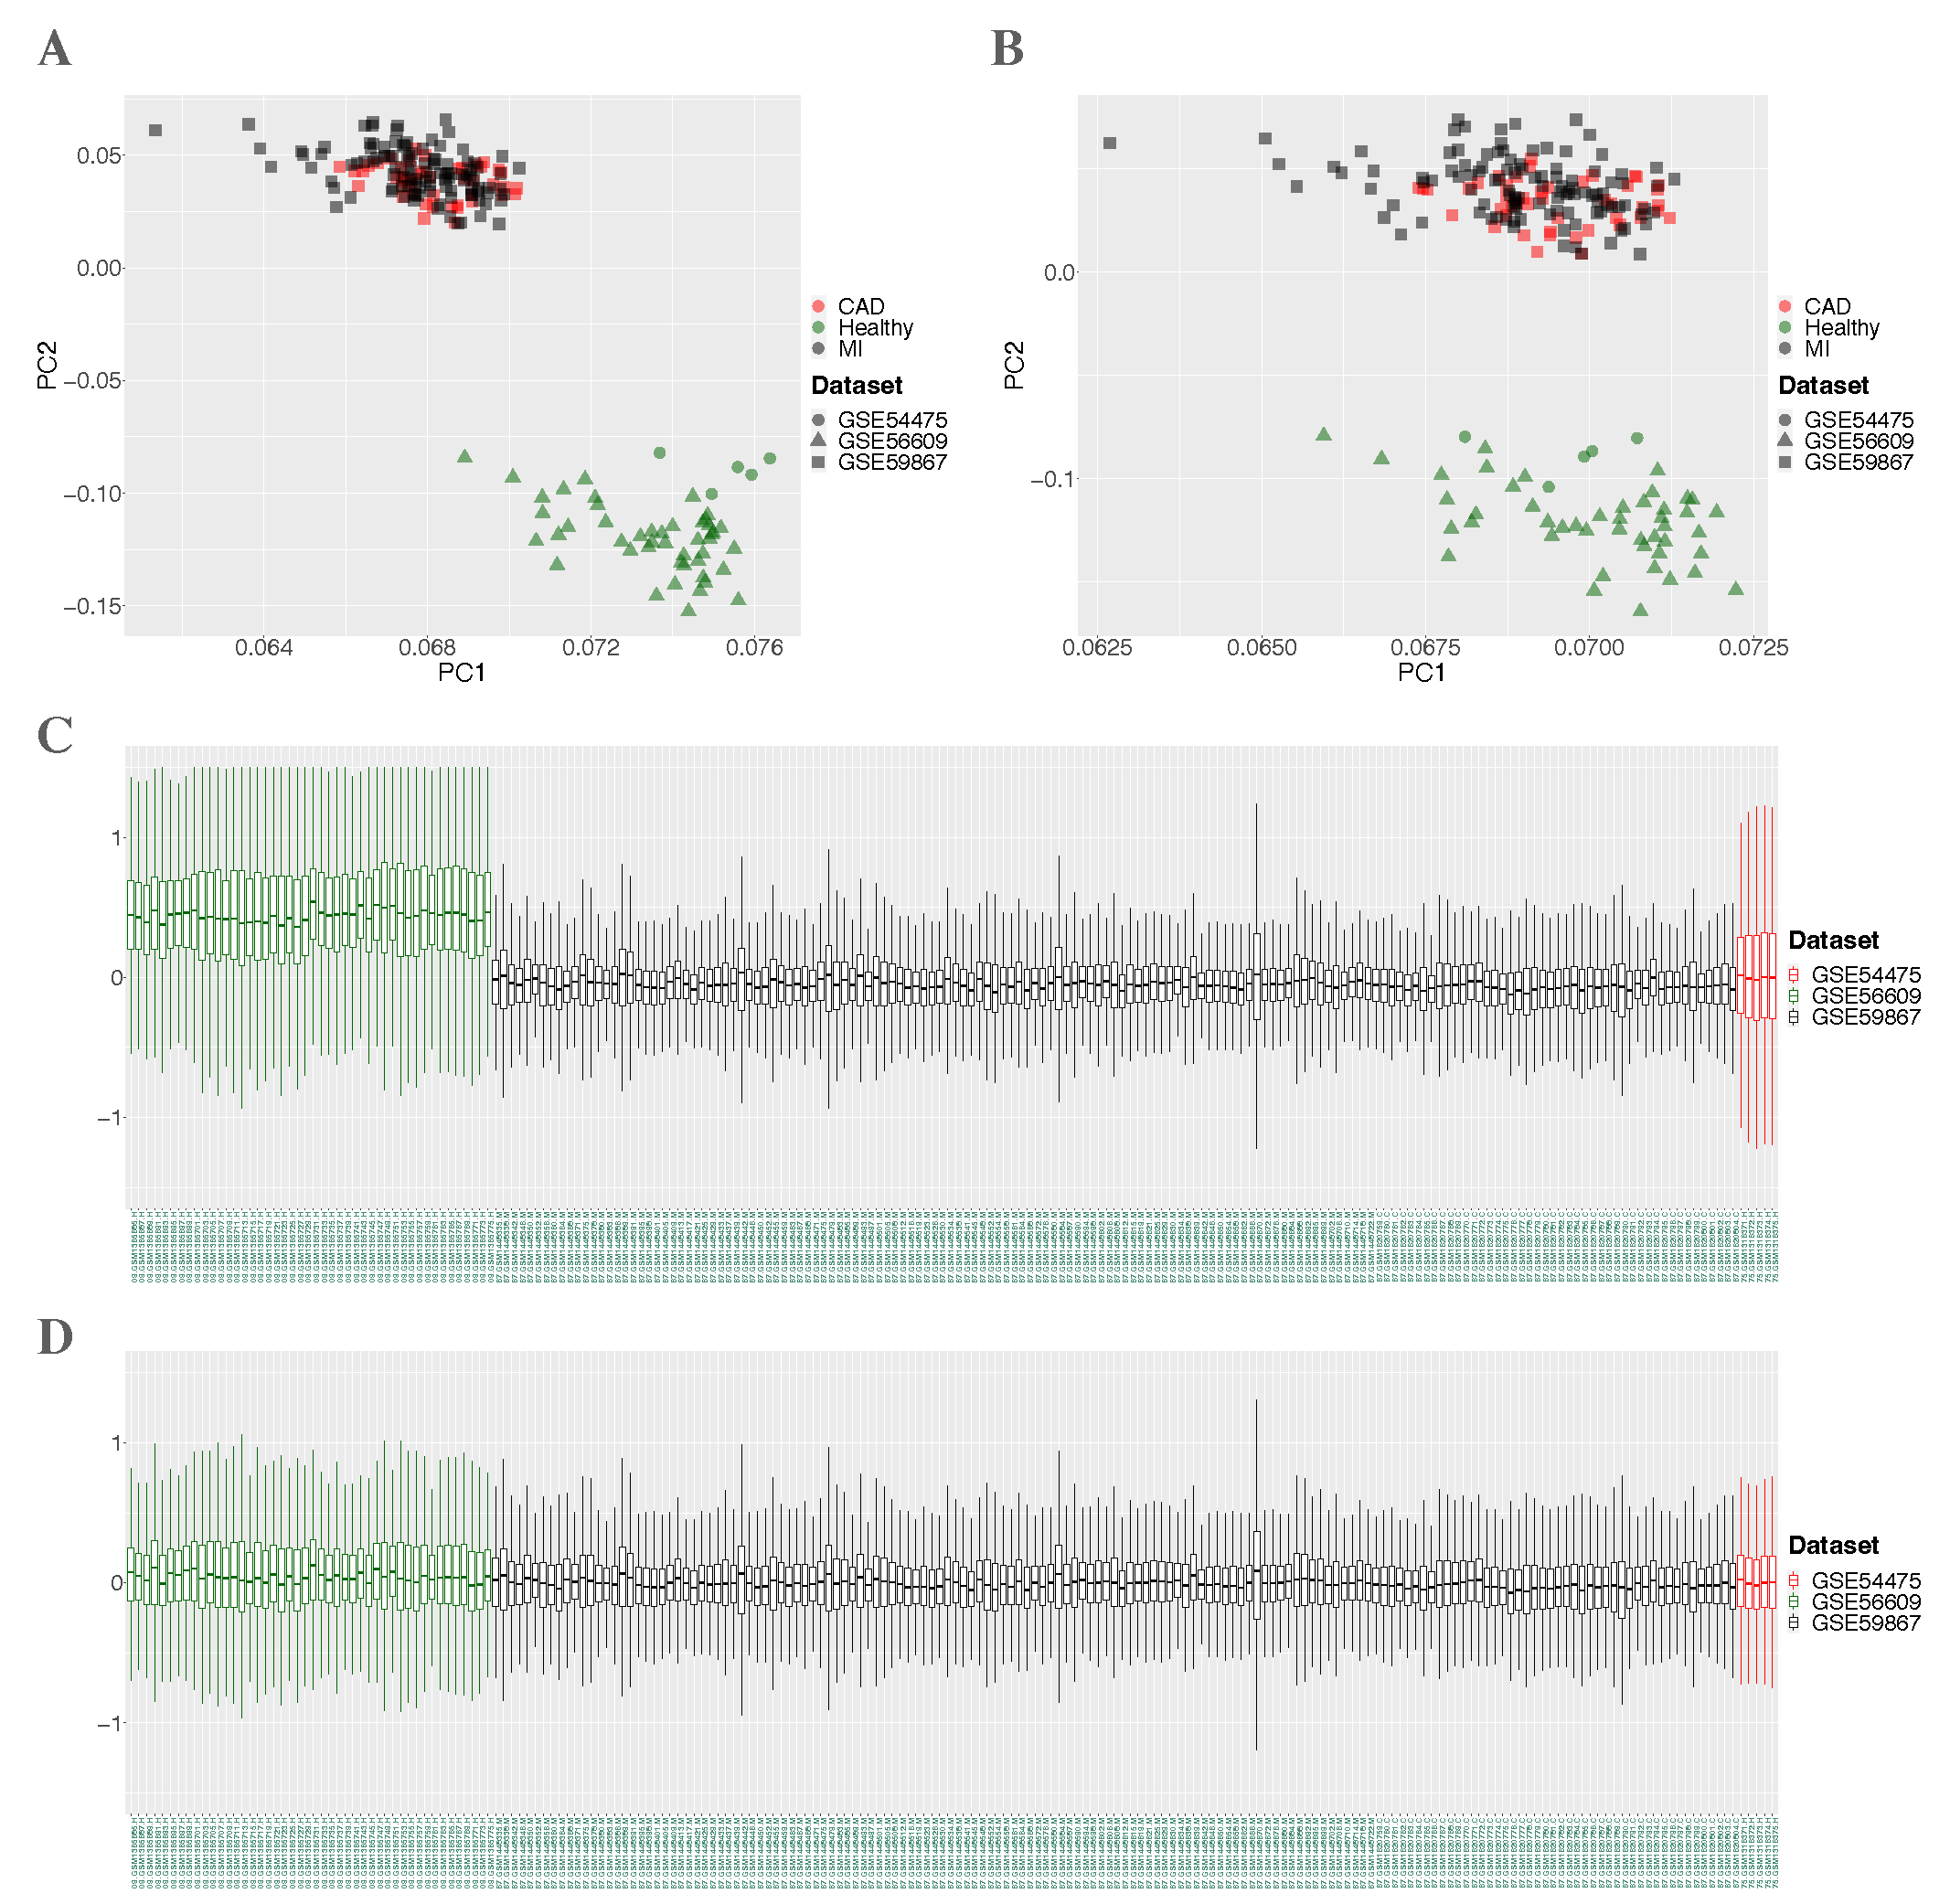
\includegraphics[width=1\linewidth]{PCA and RLE of trains} \caption{Principal component analysis plots for (A) primary data and (B) the data after fRMA, and the relative log expression plots for (C) primary data and (D) the data after fRMA.}
\label{fig:PCA}
\end{figure}

\subsection{Differential expression
analysis}\label{differential-expression-analysis-1}

\begin{table}
\centering
\caption{Total, up-, and down-regulated DEGs and differentially expressed miRNAs.}
\label{tab:DEGstab}
\begin{tabular*}{\textwidth}{@{\extracolsep\fill}lcccc}
\toprule
& Total DEGs & Up-regulated DEGs & Down-regulated DEGs & miRNAs\\
\midrule
MI vs. Healthy & 860 & 323 & 537 & miR-186, miR-21, miR-32\\
CAD vs. Healthy & 670 & 262 & 408 & miR-186, miR-21, miR-32\\
MI vs. CAD & 260 & 144 & 116 & miR-186\\
\bottomrule
\end{tabular*}
\end{table}

According to the cutoff criterion of $FDR < 0.05$, there were 860 DEGs
between MI and healthy samples. Among them, 323 were up-regulated, and
537 were down-regulated in the MI group compared to the healthy group.
In the CAD and healthy group comparison, we found 670 DEGs, of which 262
and 408 DEGs were up- and down-regulated, respectively, in CAD samples.
In the MI and CAD groups, the number of DEGs was 260, and the numbers of
up- and down-regulated genes in MI samples were 144 and 116,
respectively, compared to CAD samples. The data are summarized in Table
~\ref{tab:DEGstab}.

\begin{figure}
\centering 
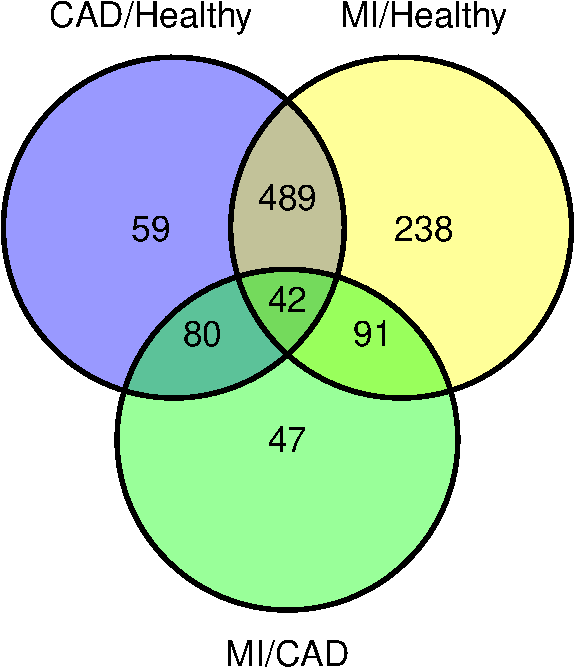
\includegraphics[width=0.45\linewidth]{venn-1}
\caption{Venn diagram for DEGs in CAD/Healthy, MI/Healthy, and MI/CAD.}\label{fig:venn}
\end{figure}

The Venn diagram in Figure~\ref{fig:venn} shows that the CAD and MI
samples shared most of their DEGs. From 860 DEGs of MI/healthy and 670
DEGs of CAD/healthy, 531 genes were common, which is 62\% of MI/healthy
DEGs and 79\% of CAD/healthy DEGs.

\subsection{GO and KEGG enrichment analyses of the
DEGs}\label{go-and-kegg-enrichment-analyses-of-the-degs}

To explore the biological classification of the DEGs, we performed GO
and KEGG pathway enrichment analyses on the MI/healthy and CAD/healthy
DEGs. For MI/healthy, GO enrichment analysis in the BP category
suggested that the DEGs were enriched in ``immune response-regulating
signaling pathway,'' ``lymphocyte differentiation,'' ``immune
response-regulating cell surface receptor signaling pathway,'' and
``leukocyte activation involved in immune response'' (Figure
~\ref{fig:MIHEnrich}A). In the CC category, DEGs were enriched in
``secretory granule membrane,'' ``azurophil granule,'' ``ficolin-1-rich
granule,'' ``tertiary granule,'' and ``ficolin-1-rich granule membrane''
(Figure~\ref{fig:MIHEnrich}B). In the MF category, DEGs were involved in
``cadherin binding'' and ``MHC class I protein binding'' (Figure
~\ref{fig:MIHEnrich}C). KEGG pathway analysis indicated that the DEGs
were related to the following pathways: ``Chemokine signaling pathway,''
``Lipid and atherosclerosis,'' and ``Hematopoietic cell lineage''
(Figure~\ref{fig:MIHEnrich}D).

\begin{figure}
\centering
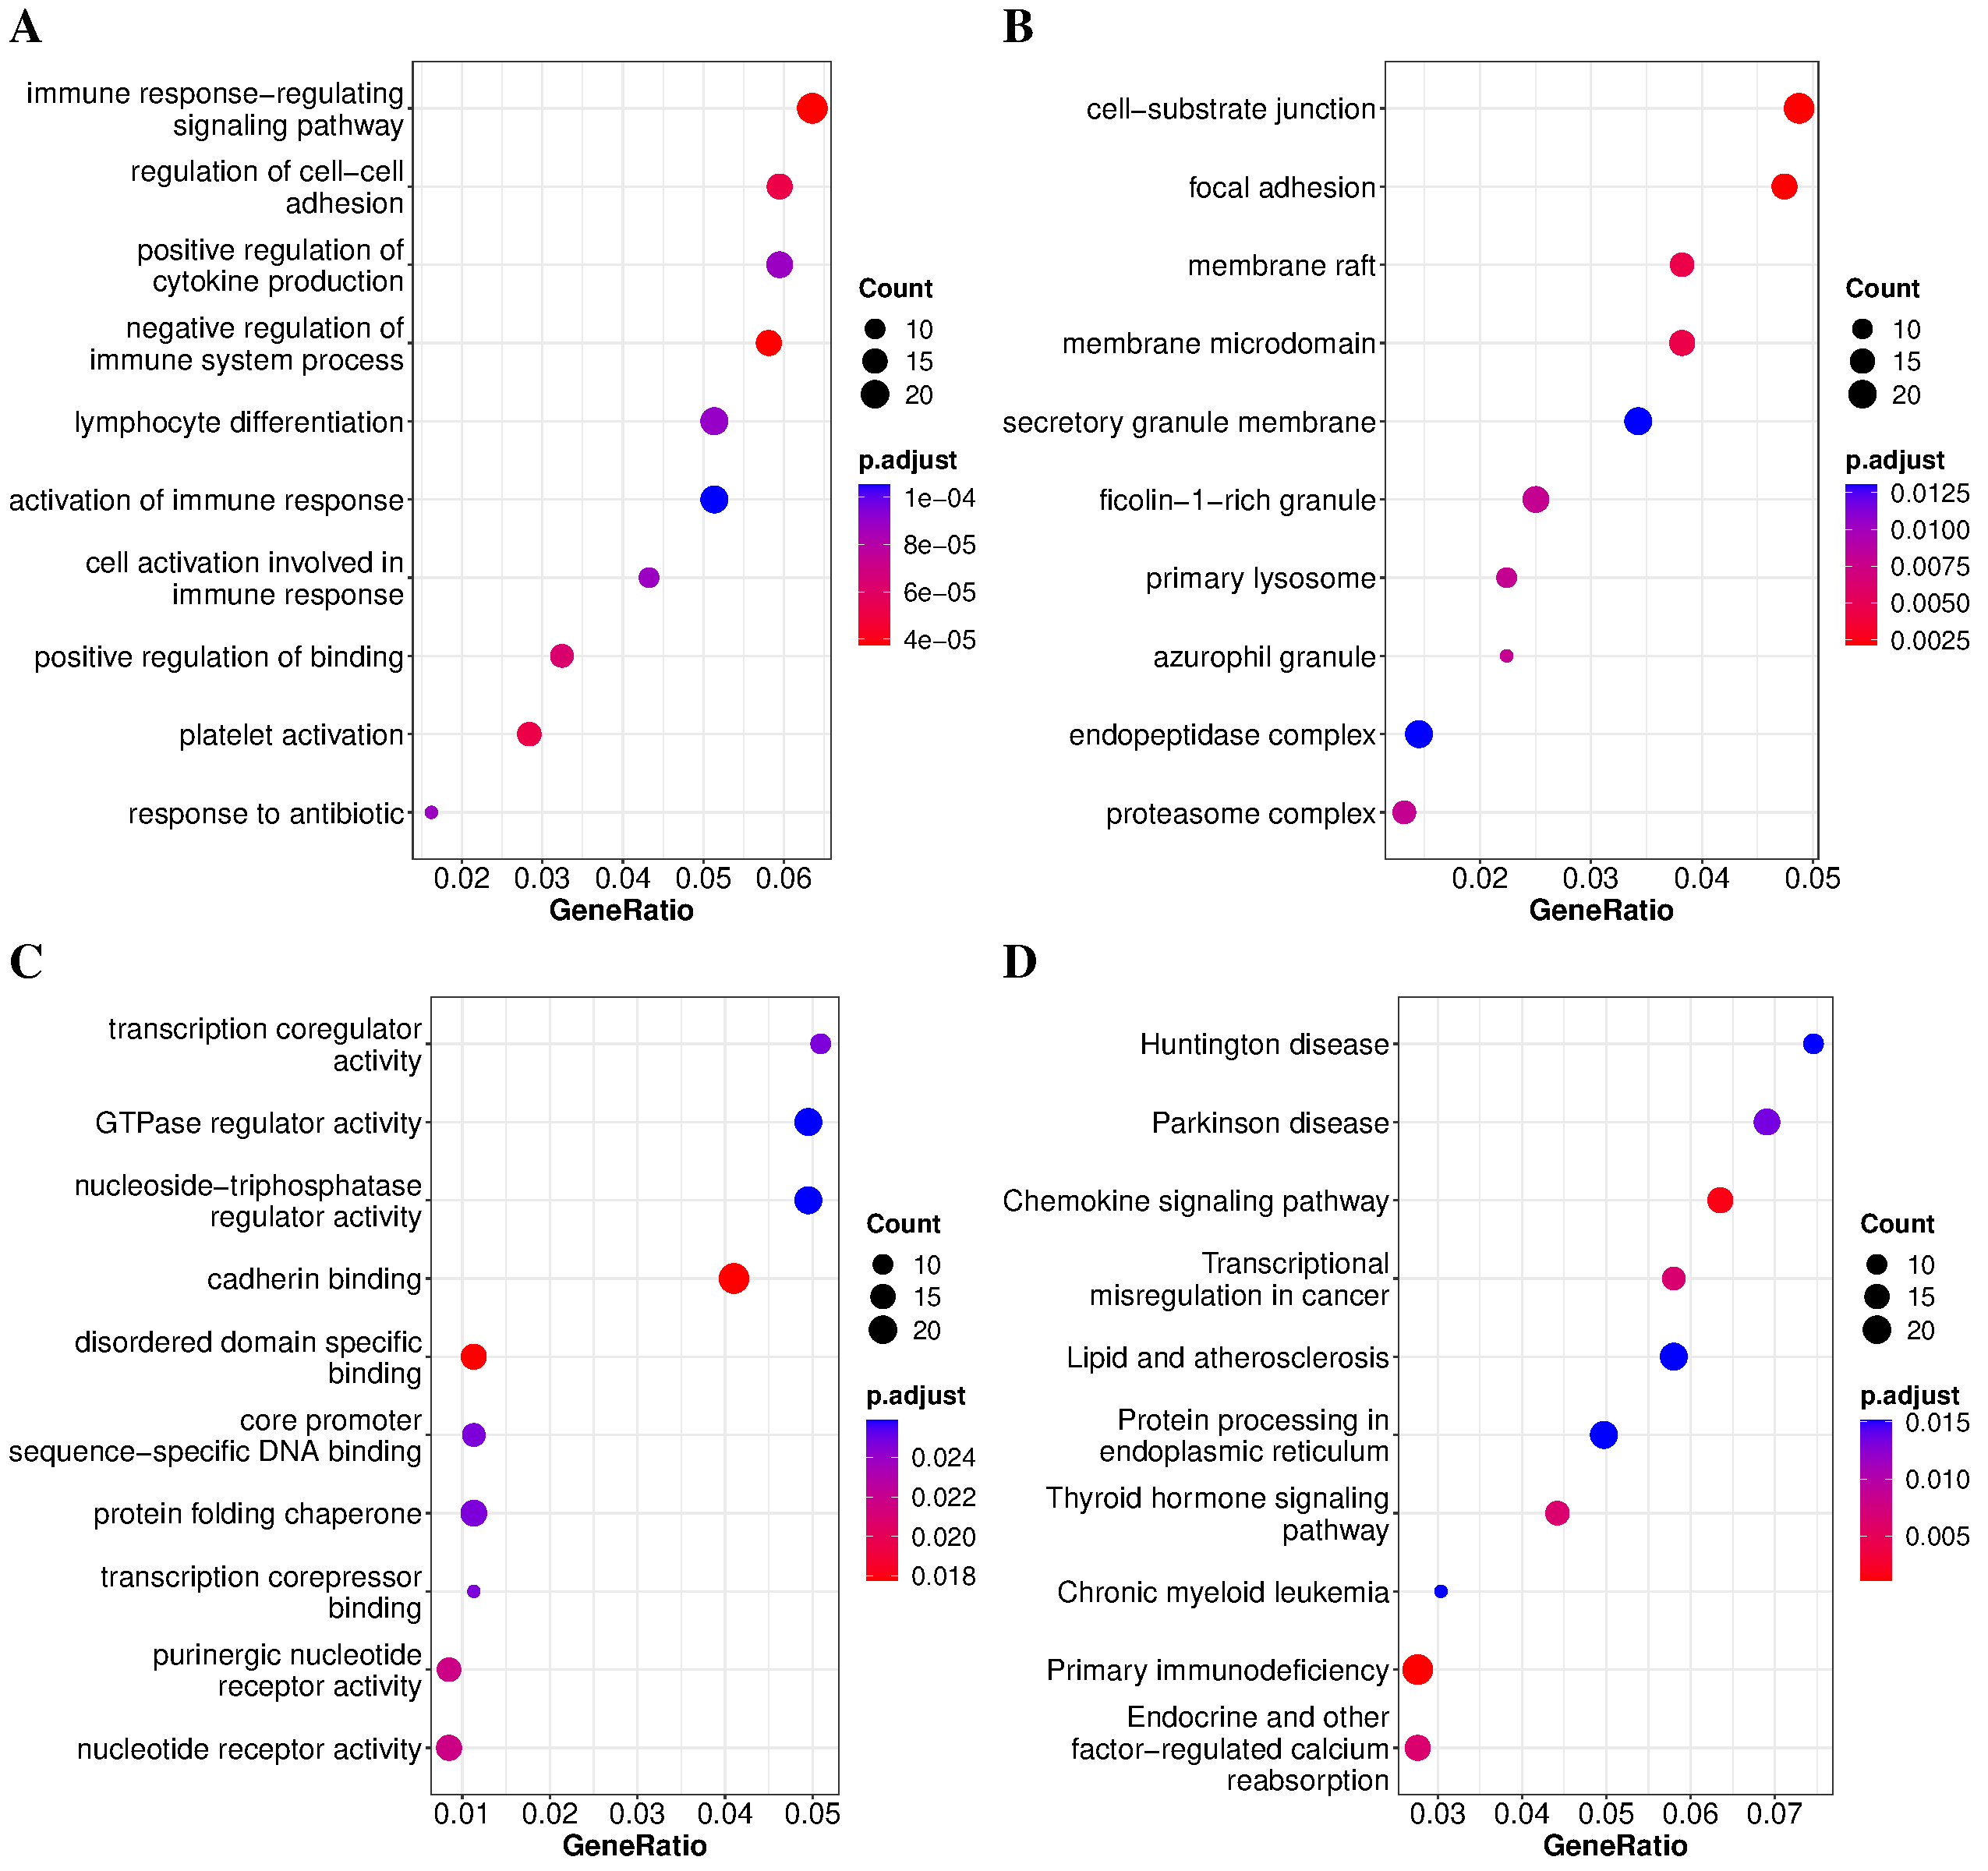
\includegraphics[width=0.95\linewidth]{Enrichment MI-Healthy} \caption{Gene Ontology (GO) and Kyoto Encyclopedia of Genes and Genomes (KEGG) pathways enriched with the MI and healthy DEGs. (A) Biological process terms. (B) Cellular component terms. (C) Molecular function terms. (D) KEGG analysis.}
\label{fig:MIHEnrich}
\end{figure}

The enrichment results for the CAD/healthy DEGs were as follows. In the
BP category, GO enrichment suggested that the DEGs were enriched in
``positive regulation of defense response,'' ``positive regulation of
innate immune response,'' ``mononuclear cell differentiation,'' and
``positive regulation of response to external stimulus'' (Figure
~\ref{fig:CADHEnrich}A). In the CC category, DEGs were enriched in
``azurophil granule,'' ``ficolin-1-rich granule,'' and ``ficolin-1-rich
granule membrane'' (Figure~\ref{fig:CADHEnrich}B). In the MF category,
DEGs were involved in ``lipoprotein particle receptor binding'' and
``NF-$\kappa$B binding'' (Figure~\ref{fig:CADHEnrich}C). KEGG pathway
analysis showed that the DEGs were related to the following pathways:
``Chemokine signaling pathway,'' ``Lipid and atherosclerosis,'' and
``Hematopoietic cell lineage'' (Figure~\ref{fig:CADHEnrich}D).

\begin{figure}
\centering
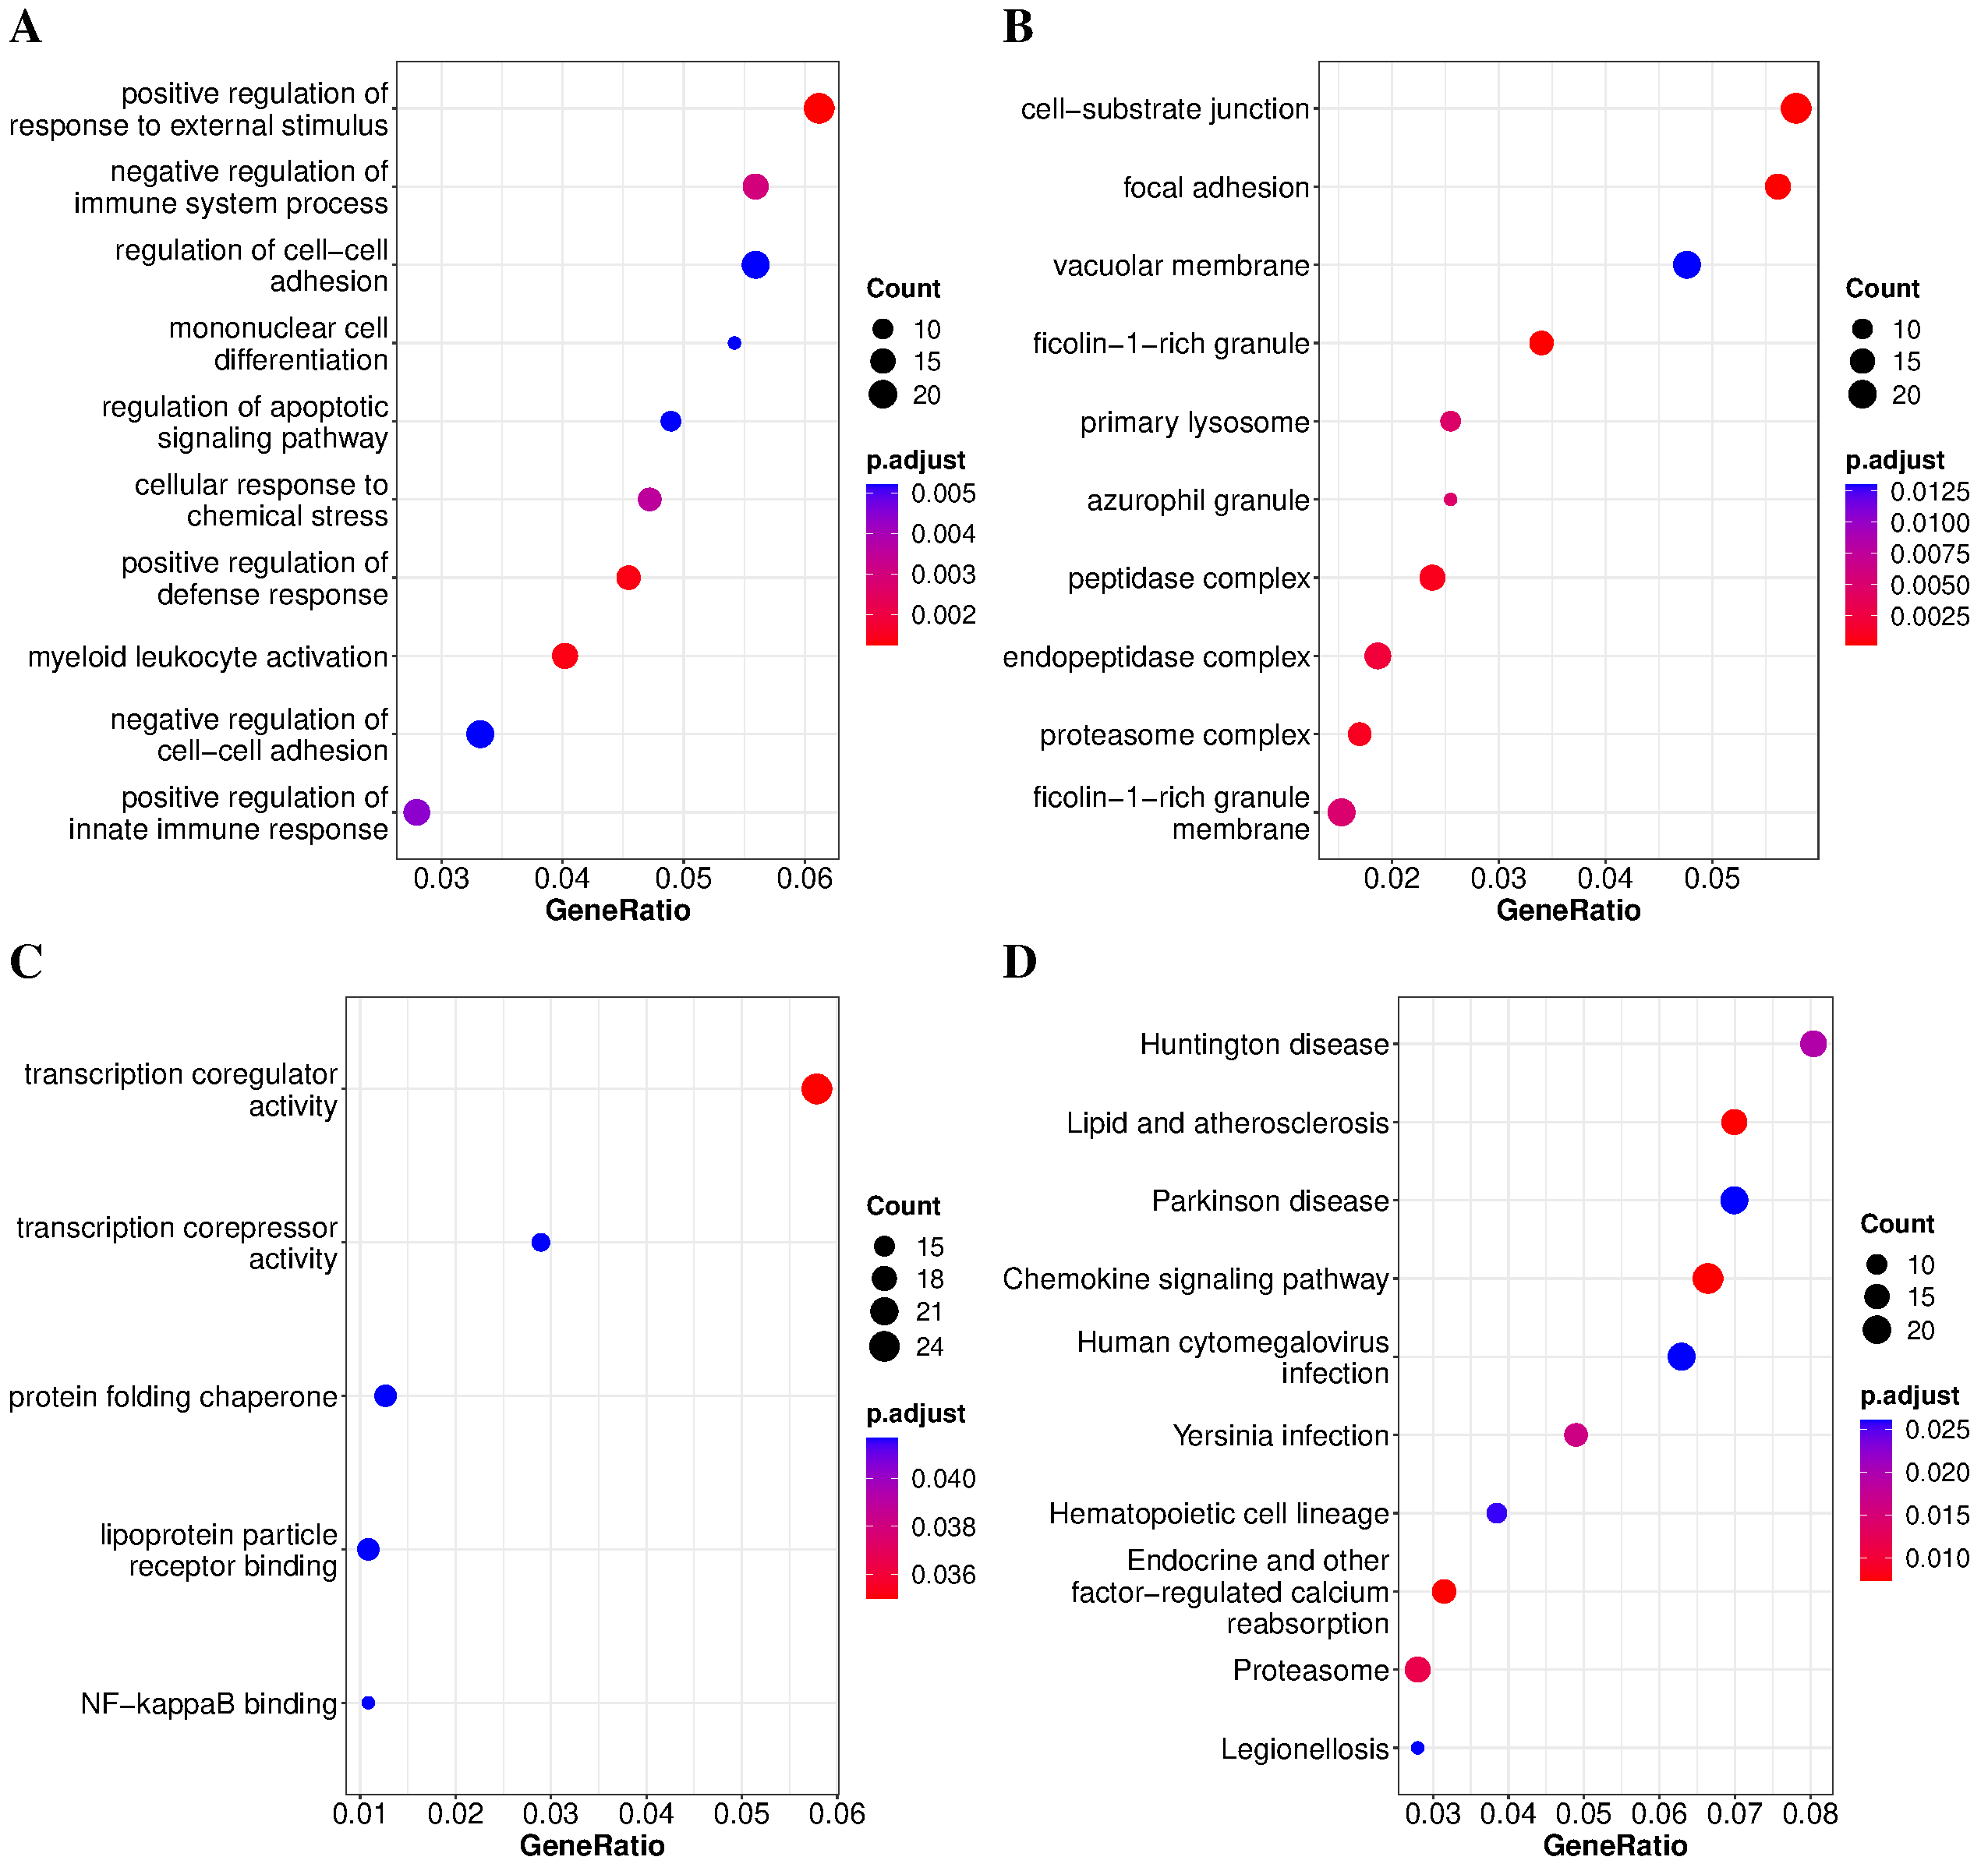
\includegraphics[width=0.95\linewidth]{Enrichment CAD-Healthy} \caption{Gene Ontology (GO) and Kyoto Encyclopedia of Genes and Genomes (KEGG) pathways enriched with the CAD and healthy DEGs. (A) Biological process terms. (B) Cellular component terms. (C) Molecular function terms. (D) KEGG analysis.}
\label{fig:CADHEnrich}
\end{figure}

\subsection{Machine Learning}\label{machine-learning}

\subsubsection{miRNAs in DEGs}\label{mirnas-in-degs-1}

Among the DEGs, miR-186, miR-32, and miR-21 were identified as
differentially expressed miRNAs. The expression profiles of the three
miRNAs are shown in Figure~\ref{fig:Expall}. The ROC curves of each
miRNA in each layer are presented in Figure~\ref{fig:miRROC}. Using the
logistic regression model, the AUC-ROC values of miR-21, miR-32, and
miR-186 for separating healthy and not-healthy samples were 0.98, 0.99,
and 0.90, respectively (Figure~\ref{fig:miRROC}A). The accuracy of each
miRNA for classifying the samples into healthy and not-healthy groups on
the test set for miR-21, miR-32, and miR-186 was 0.92, 0.98, and 0.89,
respectively. The ROC curve of each miRNA for classifying MI and CAD
samples is presented in Figure~\ref{fig:miRROC}B. The AUC-ROC and
accuracy for miR-21, miR-32, and miR-186 in the test set were 0.85;
0.70; and 0.86, and 0.78; 0.67; and 0.74, respectively.

\begin{table}
\centering
\caption{Investigated miRNAs log fold-change and adjusted p-values for CAD samples relative to healthy, MI samples relative to healthy, and MI samples relative to CAD.}
\label{tab:mirExptable}
\begin{tabular}{lcccccc}
\toprule
\multicolumn{1}{c}{} & \multicolumn{2}{c}{CAD/Healthy} & \multicolumn{2}{c}{MI/Healthy} & \multicolumn{2}{c}{MI/CAD} \\
\cmidrule(lr){2-3} \cmidrule(lr){4-5} \cmidrule(lr){6-7}
& logFC & adj. p-value & logFC & adj. p-value & logFC & adj. p-value\\
\midrule
miR-186 & 1.4 & 3.60e-25 & 0.9 & 6.76e-20 & -0.5 & 1.05e-09\\
miR-21 & 1.4 & 1.31e-17 & 2.3 & 2.07e-47 & 0.8 & 2.96e-11\\
miR-32 & 2.5 & 8.39e-43 & 2.2 & 3.10e-59 & -0.3 & 7.60e-04\\
miR-197 & 0.5 & 2.95e-20 & 0.7 & 1.59e-47 & 0.2 & 8.58e-09\\
miR-29A & 0.7 & 7.76e-29 & 0.1 & 1.70e-01 & -0.5 & 2.14e-10\\
miR-296 & -0.1 & 5.00e-02 & 0.1 & 2.00e-02 & 0.2 & 6.15e-06\\
\bottomrule
\end{tabular}
\end{table}

\begin{figure}
\centering 
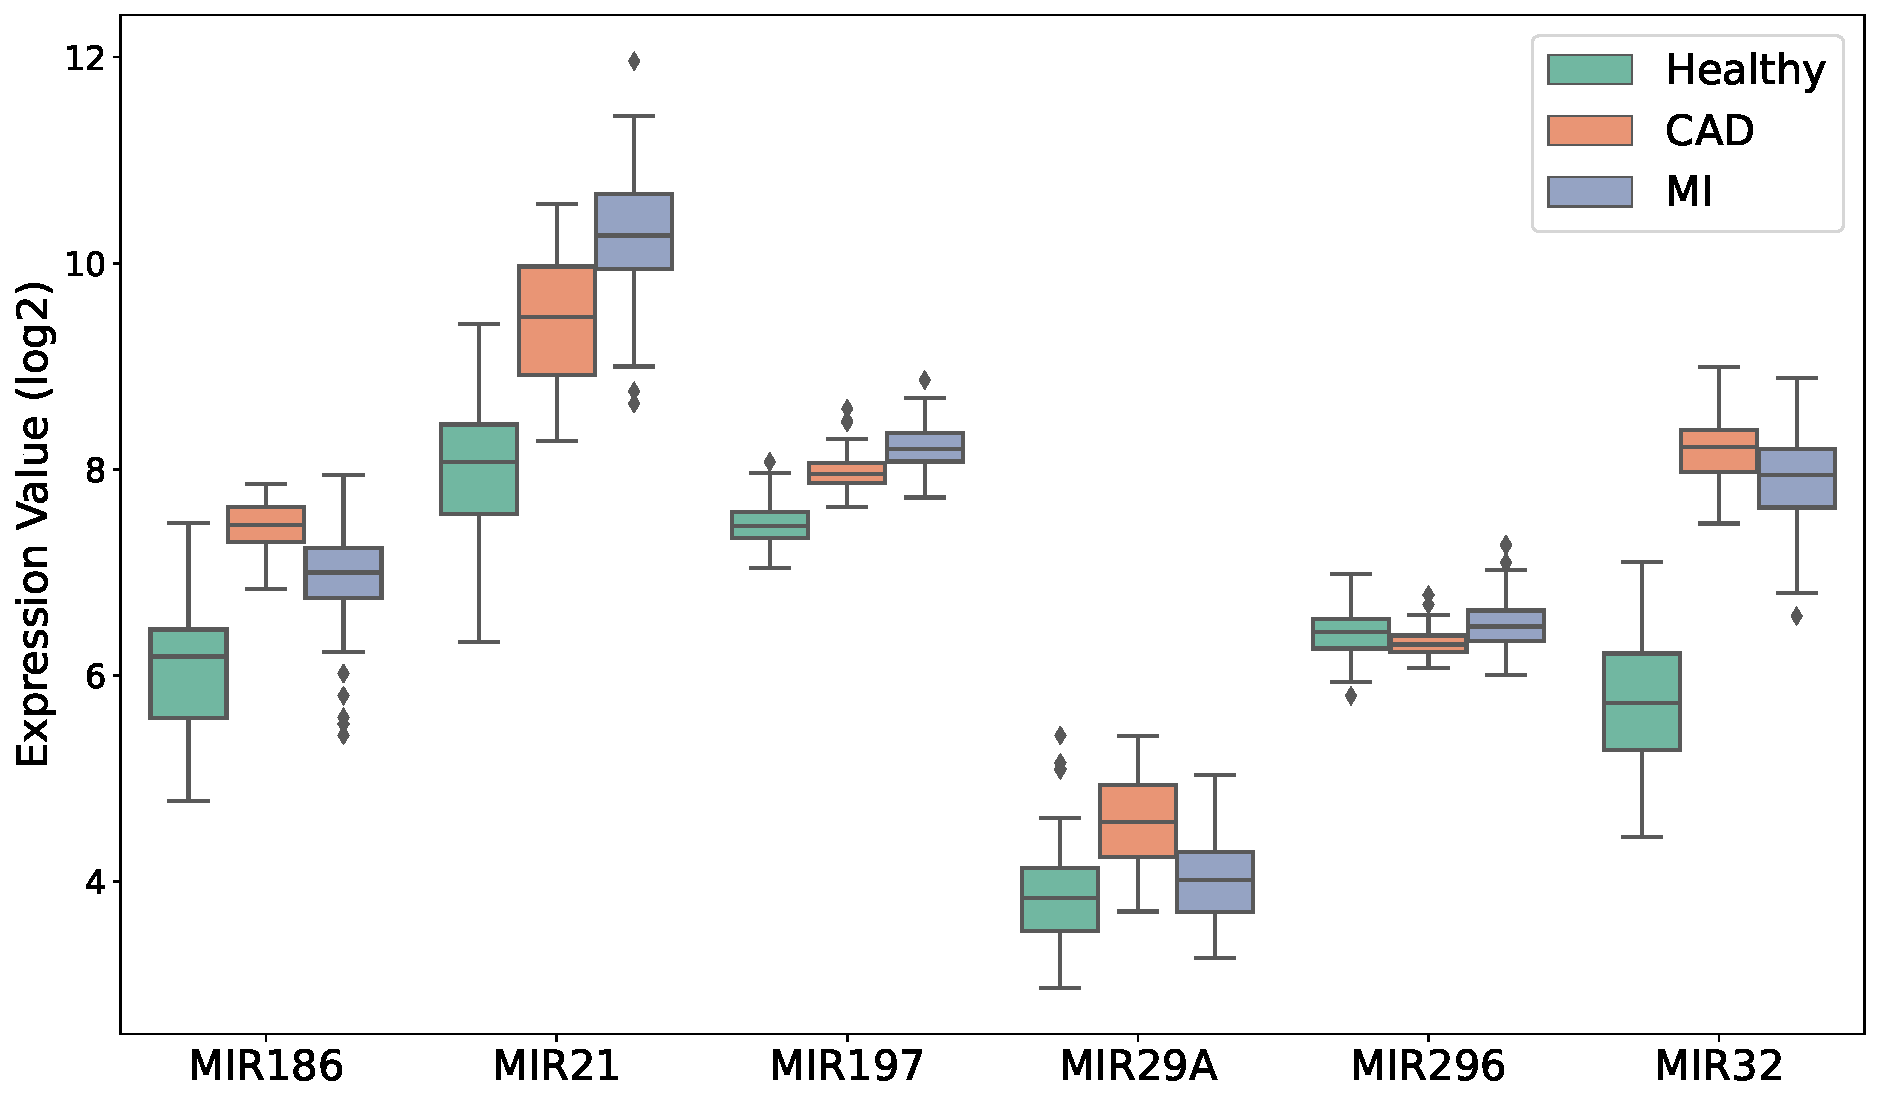
\includegraphics[width=0.9\linewidth]{Expressionforall}
\caption{Expression profile of all miRNAs in two approaches in different sample classes.}\label{fig:Expall}
\end{figure}

\begin{figure}
\centering 
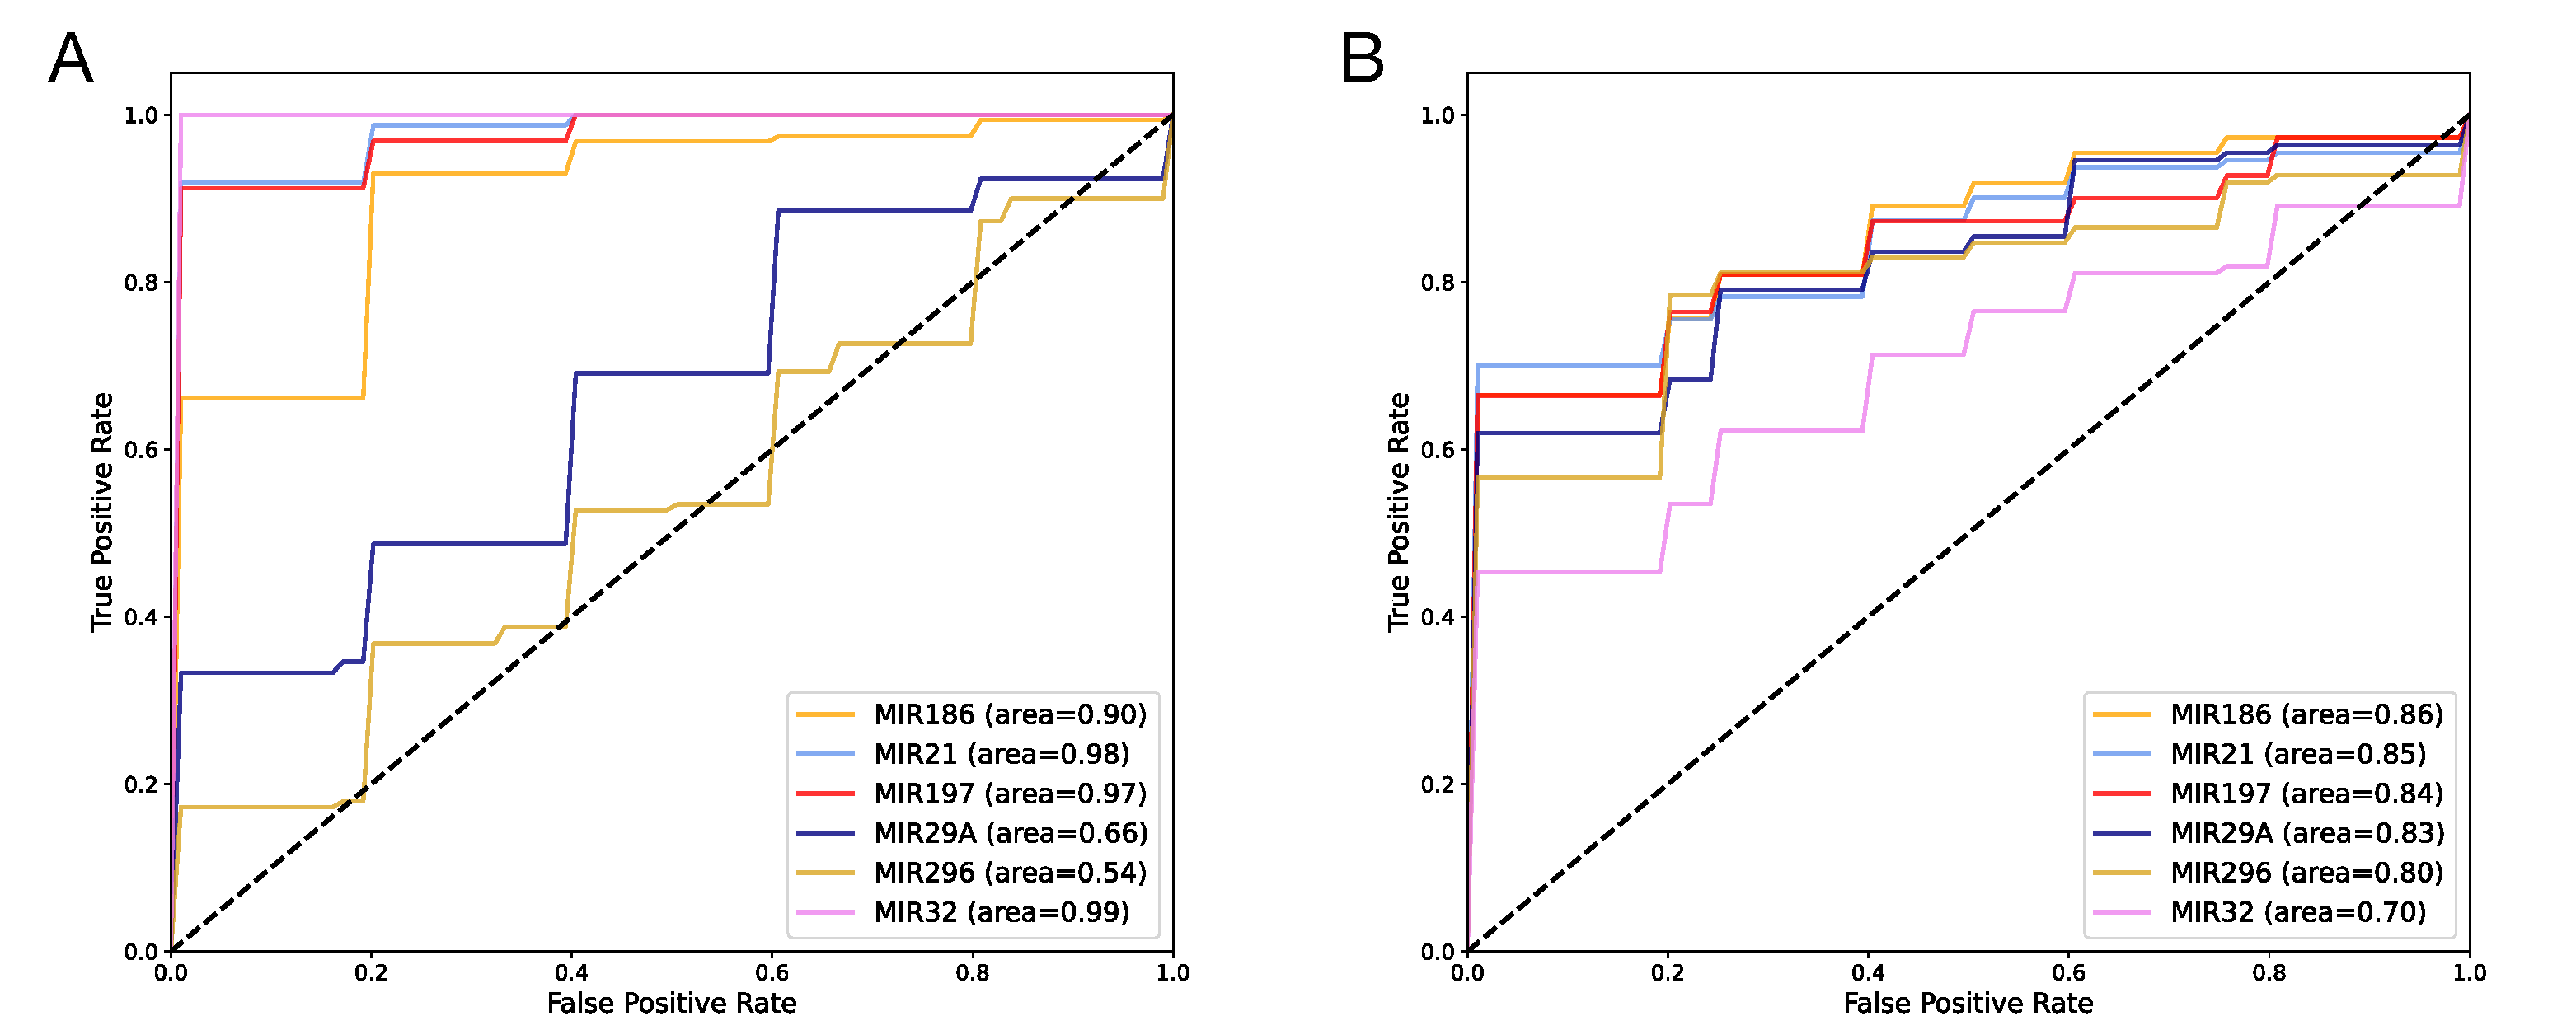
\includegraphics[width=0.95\linewidth]{miRs ROCs}
\caption{ROC curve for single miRNAs on test set classification for (A) healthy and not-healthy samples and (B) CAD and MI samples.}\label{fig:miRROC}
\end{figure}

\paragraph{First layer for the isolation of healthy and not-healthy
samples:}\label{first-layer-for-the-isolation-of-healthy-and-not-healthy-samples-2}

Although single miRNAs had an acceptable performance for this layer,
their predictive value could be further improved by using them as a set.
The ROC curve for the SVM model with an RBF kernel trained with all
three miRNAs is presented in Figure~\ref{fig:DEMROC}A. The model had a
better performance in classification than single miRNAs.The AUC-ROC for
the model was 1, and its accuracy on the test set was also 1. In Figure
~\ref{fig:DEMCF}A, the confusion matrix for the model is presented.

\begin{figure}
\centering 
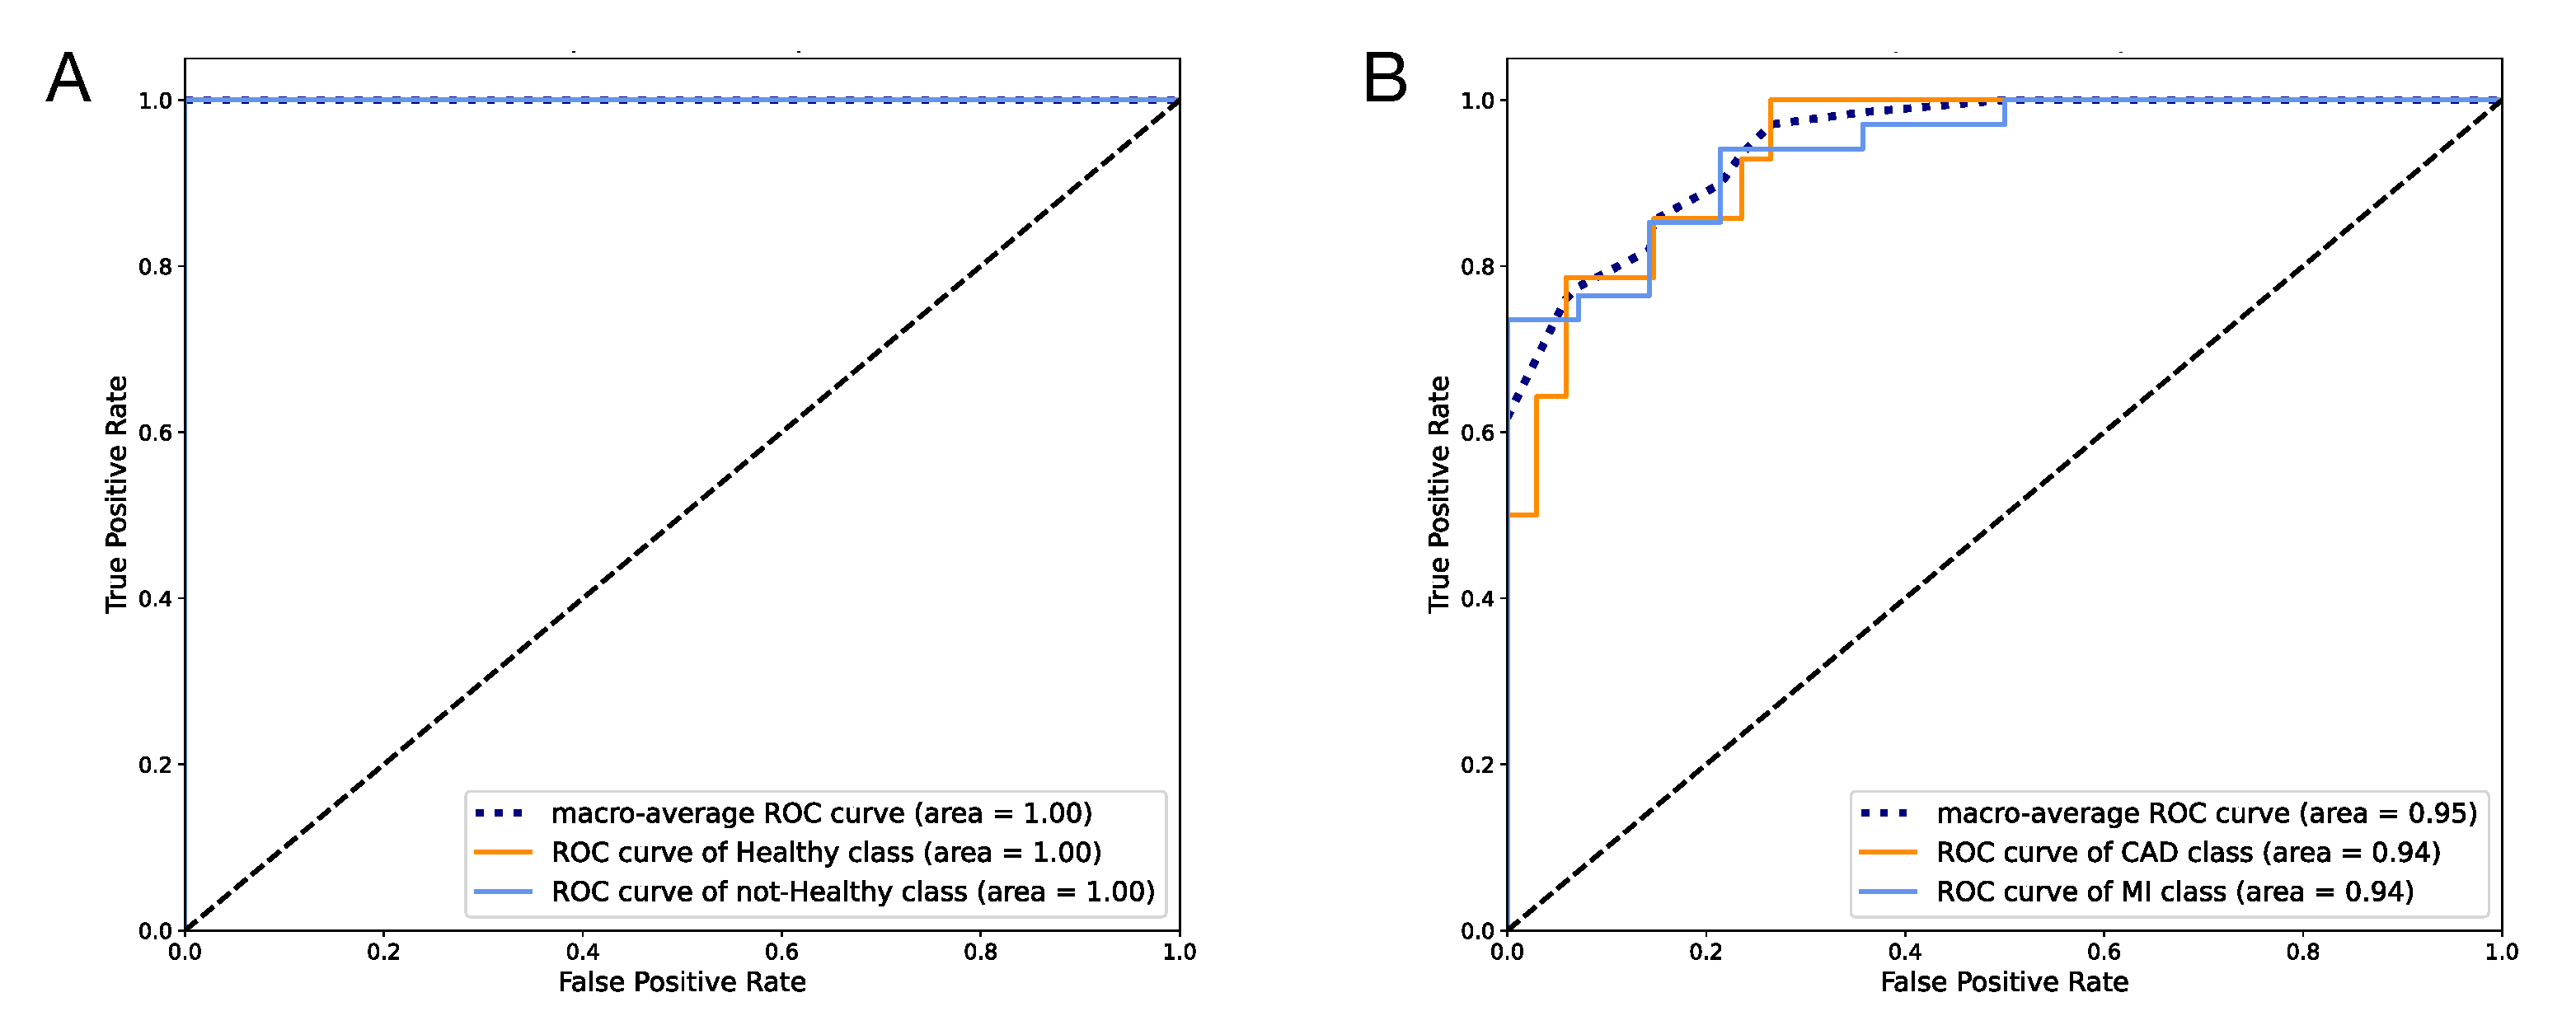
\includegraphics[width=0.95\linewidth]{DEMs ROCs h not h cad mi}
\caption{ROC curve for the model trained with miRNAs in DEGs on test set classification; (A) An SVM model with RBF kernel for healthy and not-healthy and (B) An SVM model with linear kernel for CAD and MI sample classification.}\label{fig:DEMROC}
\end{figure}

\begin{figure}
\centering 
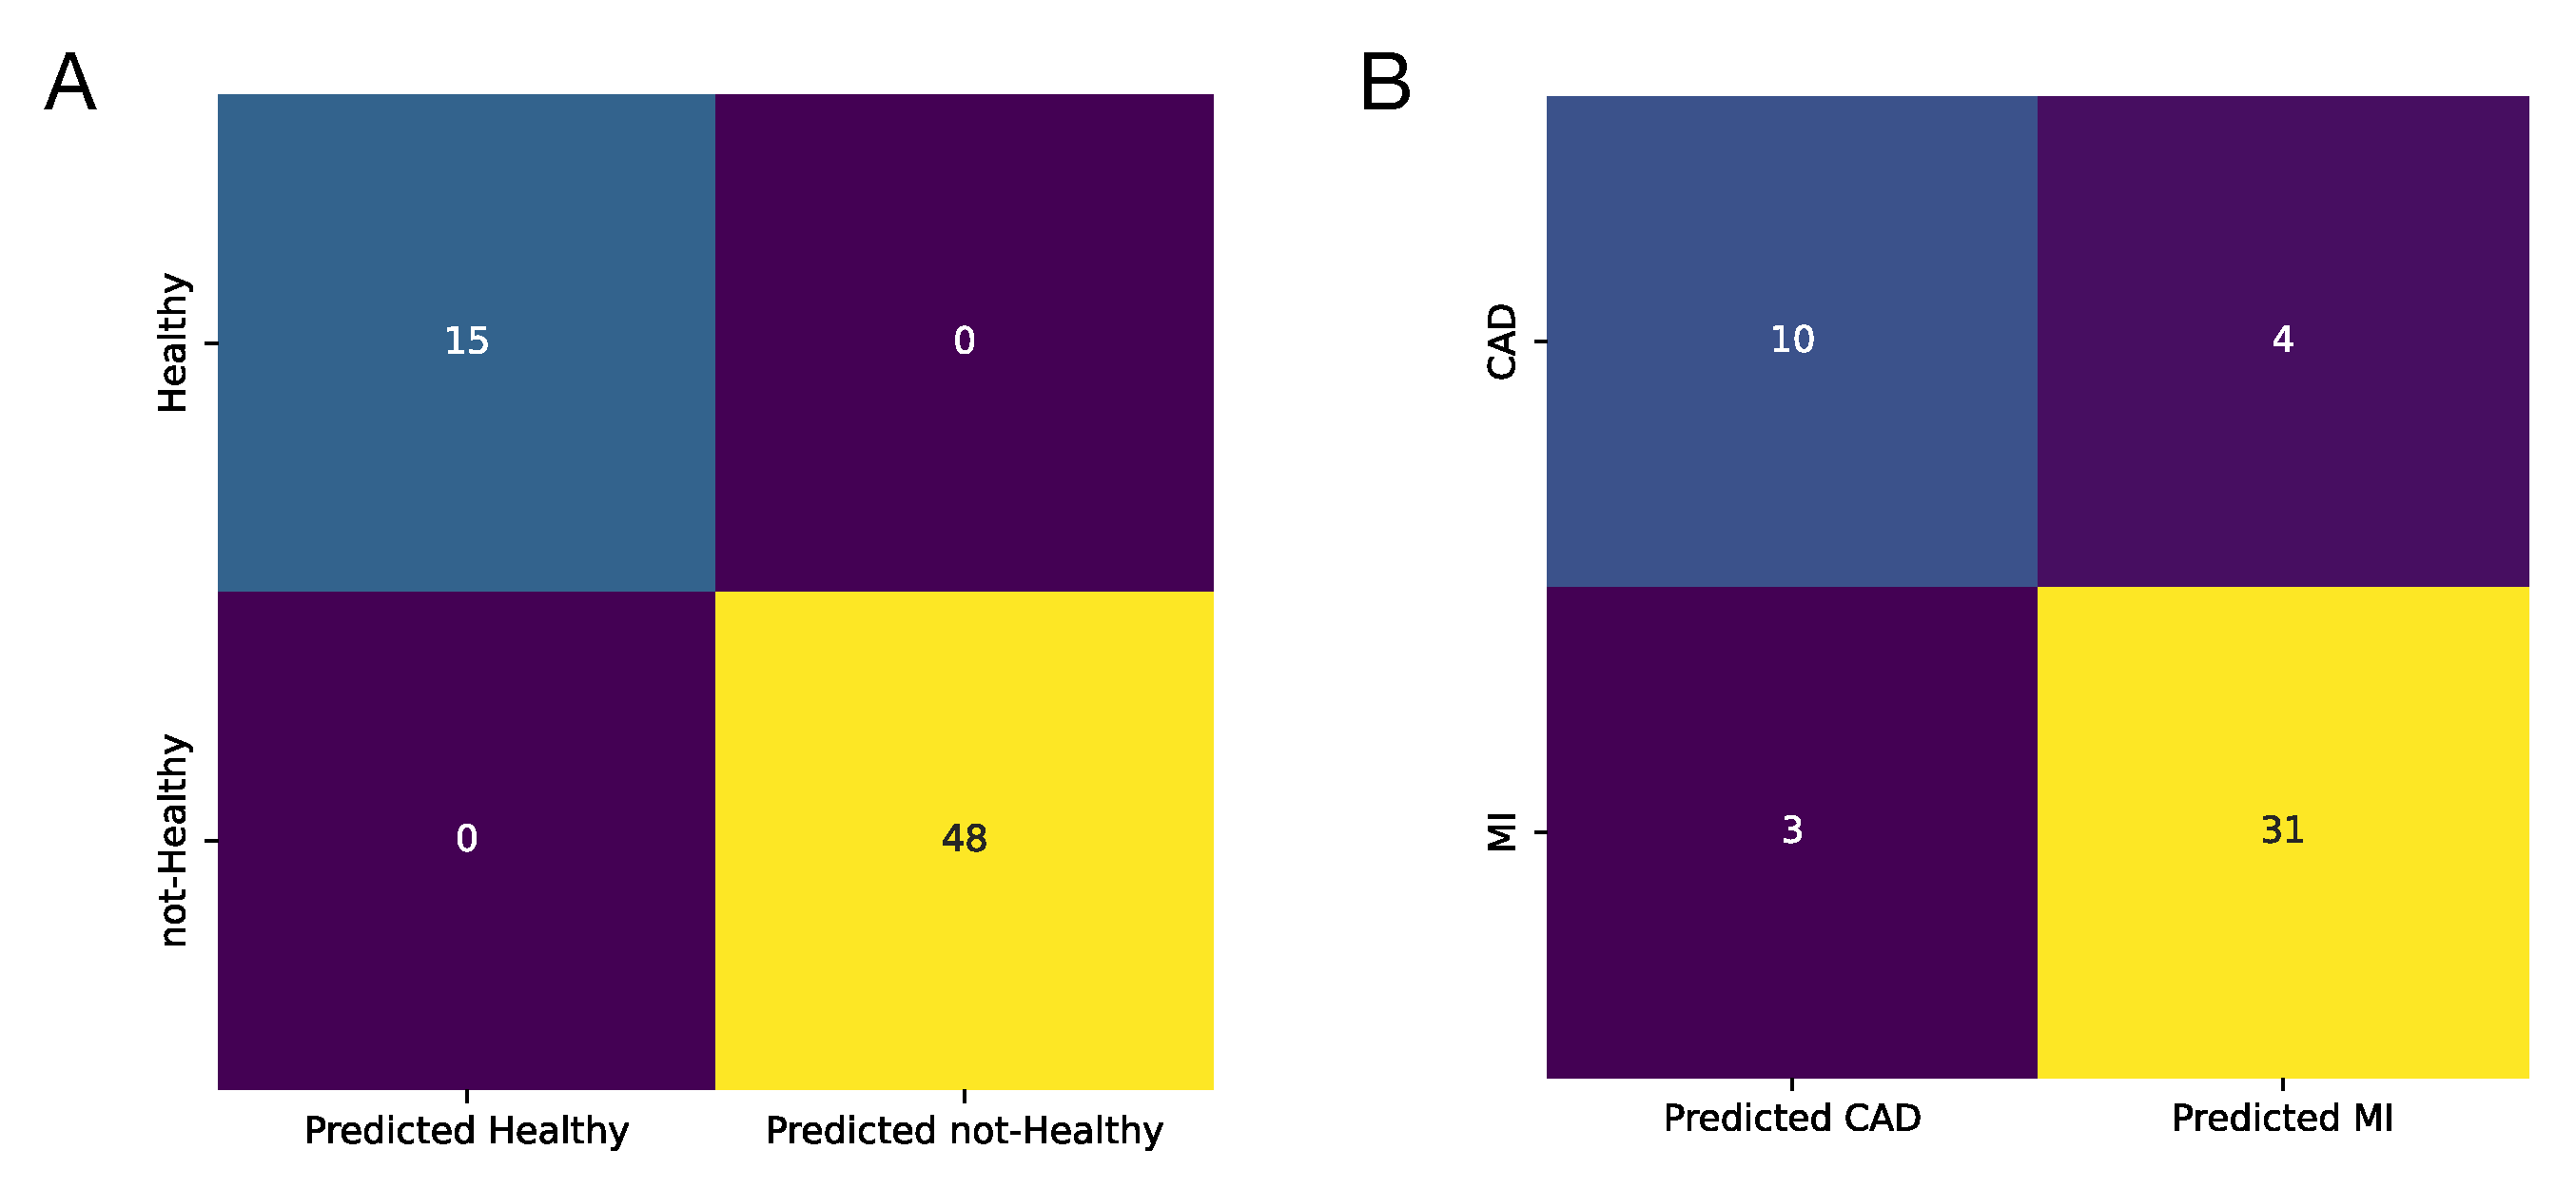
\includegraphics[width=0.9\linewidth]{DEMs Conf. matrix}
\caption{Confusion matrix for the model trained with miRNAs in DEGs on test set classification; (A) An SVM model with RBF kernel for healthy and not-healthy and (B) An SVM model with linear kernel for CAD and MI sample classification.}\label{fig:DEMCF}
\end{figure}

\paragraph{Second layer for separating the MI and CAD
samples:}\label{second-layer-for-separating-the-mi-and-cad-samples-2}

Different models were trained using the expression values of three
differentially expressed miRNAs. The models' AUC-ROC and the accuracy of
the test set are shown in Figure~\ref{fig:DEMmodels}. The best model
from both the AUC-ROC and accuracy points of view was the SVM model with
a linear kernel. The AUC-ROC and accuracy for this model with its preset
values were 0.93 and 0.82, respectively. The model was hypertuned for C
and gamma hyperparameters, and therefore the model showed better
performance. The ROC curve of the hypertuned model is presented in
Figure~\ref{fig:DEMROC}B. For this model, the AUC-ROC reached 0.95, and
the accuracy was improved to 0.85 (Table~\ref{tab:DEGsML}). Moreover,
the sensitivity and specificity for the model on the test set were 0.91
and 0.71, respectively. The confusion matrix for the hypertuned model is
illustrated in Figure~\ref{fig:DEMCF}B.

\begin{figure}
\centering
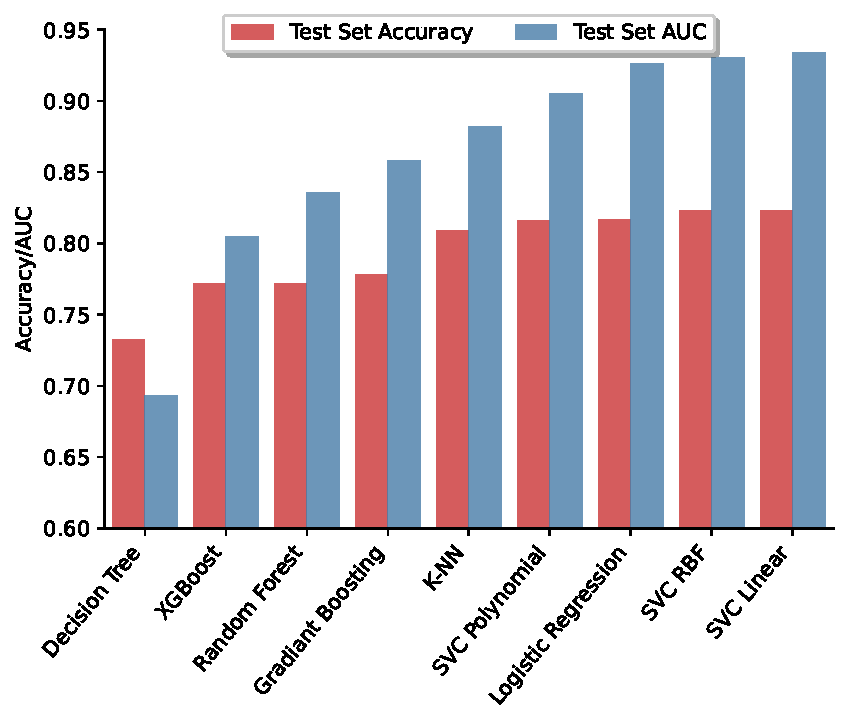
\includegraphics[width=0.65\linewidth]{Models DEGs mirs}
\caption{Area under the receiver operating characteristic curve and accuracy of different models trained with three miRNAs in DEGs.}\label{fig:DEMmodels}
\end{figure}


\begin{table}
\centering
\caption{AUC-ROC and accuracy for SVM with a linear kernel as the best model trained with differentially expressed miRNAs on the training and test sets before and after hypertuning}
\label{tab:DEGsML}
\begin{tabular}{cccccc}
\toprule
\multicolumn{2}{c}{} & \multicolumn{2}{c}{Preset parameters} & \multicolumn{2}{c}{Hypertuned} \\
\cmidrule(lr){3-4} \cmidrule(lr){5-6}
Model & Metrics & train & test & train & test\\
\midrule
SVM-linear & AUC-ROC & 0.91 & 0.93 & 0.92 & 0.95\\
& Accuracy & 0.83 & 0.82 & 0.84 & 0.85\\
\bottomrule
\end{tabular}
\end{table}

\subsubsection{AUC-ROC approach}\label{auc-roc-approach}

After calculating the AUC-ROC for each miRNA to classify of MI and CAD
samples, the miRNAs with AUC-ROC $> 0.8$ were selected. The miRNAs
selected were miR-29a, miR-197, miR-186, miR-21, and miR-296. The
expression levels of these miRNAs in healthy, CAD, and MI samples are
presented in Figure~\ref{fig:Expall}. The ROC curves of the selected
miRNAs in both layers are shown in Figure~\ref{fig:miRROC}.

\paragraph{First layer for the isolation of healthy and not-healthy
samples:}\label{first-layer-for-the-isolation-of-healthy-and-not-healthy-samples-3}

Using the selected set, an SVM model with an RBF kernel was trained to
separate healthy and not-healthy samples. The ROC curve for the model is
presented in Figure~\ref{fig:AUCROC}A, and the confusion matrix is
illustrated in Figure~\ref{fig:AUCCF}A. Both the AUC-ROC and accuracy of
the model on the test set were 1.

\begin{figure}
\centering 
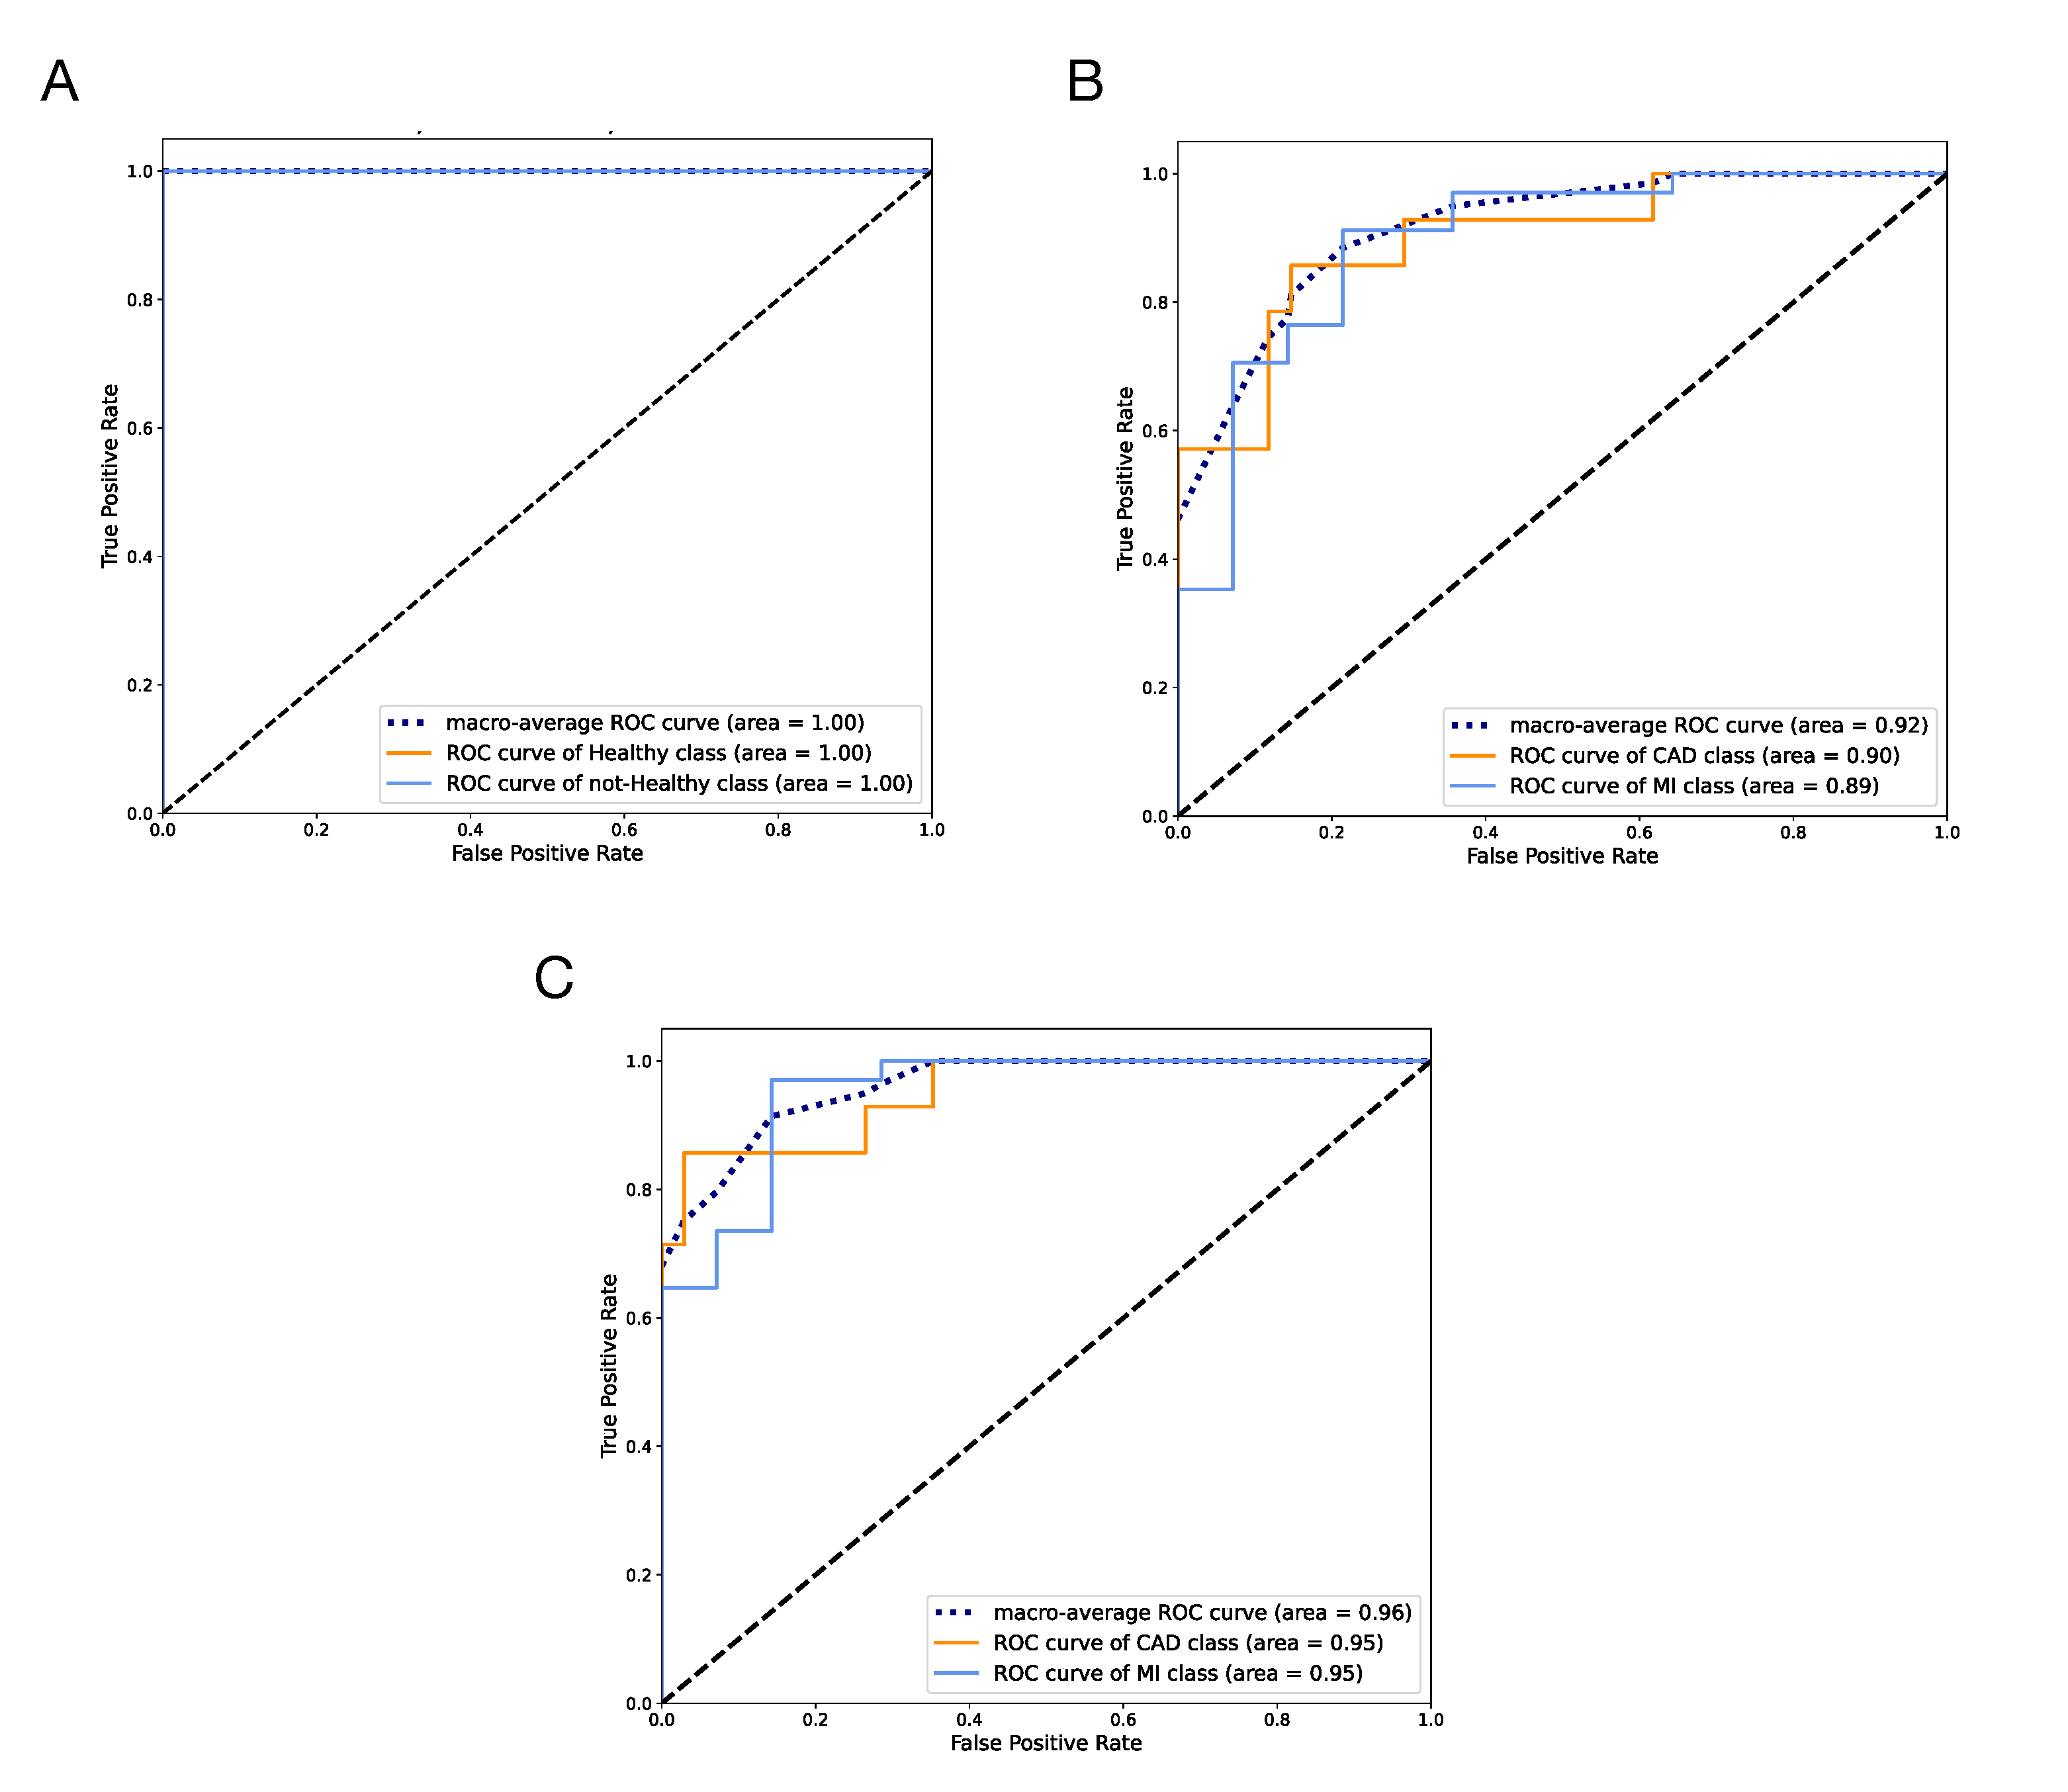
\includegraphics[width=0.95\linewidth]{AUC best model ROCs}
\caption{ROC curve for models trained with the set of miRNAs selected by AUC-ROC on test set classification; (A) SVM with RBF kernel for healthy and not-healthy samples classification. (B) Logistic regression model for CAD and MI sample classification. (C) SVM with polynomial kernel for CAD and MI sample classification. }\label{fig:AUCROC}
\end{figure}

\begin{figure}
\centering 
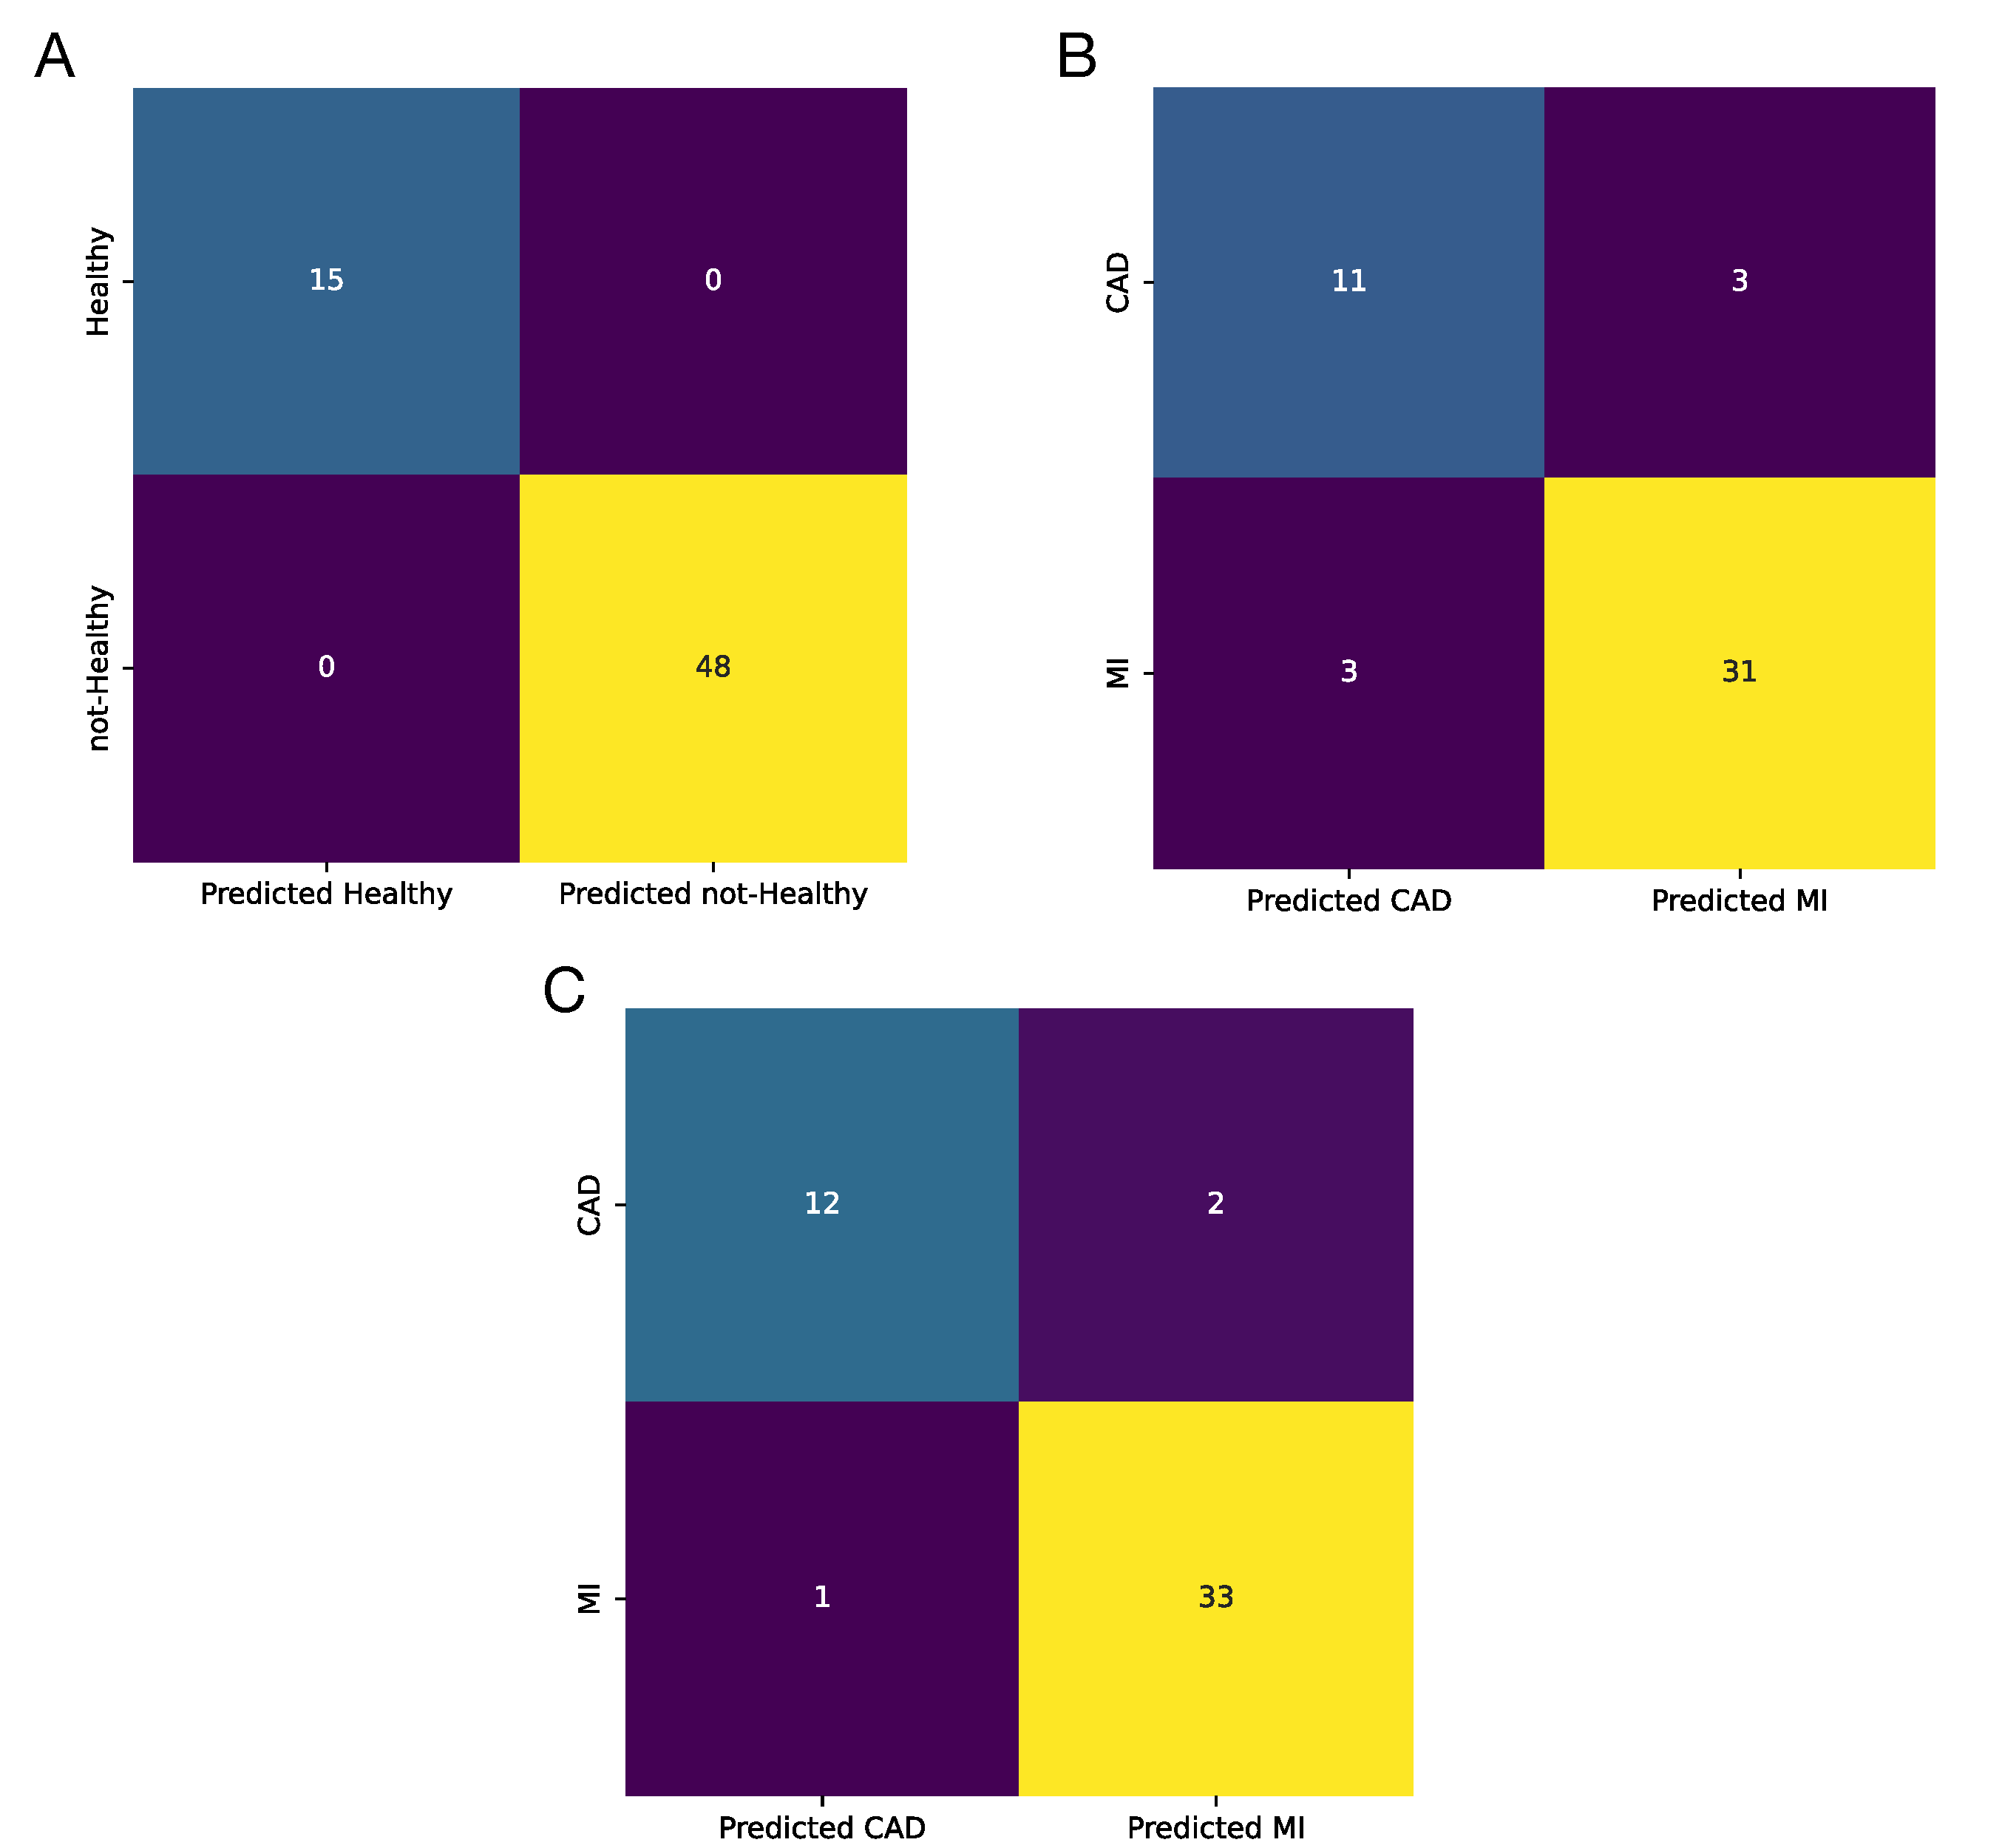
\includegraphics[width=0.9\linewidth]{AUC Conf. matrix}
\caption{Confusion matrix for models trained with the set of miRNAs selected by AUC-ROC on test set classification; (A) SVM with RBF kernel for healthy and not-healthy samples classification. (B) Logistic regression model for CAD and MI sample classification. (C) SVM with polynomial kernel for CAD and MI sample classification.}\label{fig:AUCCF}
\end{figure}

\paragraph{Second layer for separating the MI and CAD
samples:}\label{second-layer-for-separating-the-mi-and-cad-samples-3}

To find the best model for this set of miRNAs, different models were
trained using their preset values. The AUC-ROC and accuracy results for
the test set are presented in Figure~\ref{fig:AUCmodels}. The best model
from the AUC-ROC point of view was the SVM with a linear kernel, and
from the accuracy point of view, it was the SVM model with an RBF
kernel. For the SVM-linear model, the AUC-ROC and accuracy were 0.93 and
0.82, respectively; and for the SVM-RBF, the values were 0.92 and 0.84,
respectively. Both models were hyper-tuned, and the ROC curve for their
best performance is presented in Figure~\ref{fig:AUCROC}B and C. The
AUC-ROC and accuracy for the SVM-linear model were modified to 0.92 and
0.88, respectively. For the SVM-RBF, these values increased to 0.96 and
0.94, respectively (Table~\ref{tab:AUCML}). The sensitivities for the
SVM-linear and SVM-RBF models were 0.91 and 0.97, respectively; and
their specificities were 0.79 and 0.86, respectively. The confusion
matrix for both models is illustrated in Figure~\ref{fig:AUCCF}B and C.

\begin{figure}
\centering 
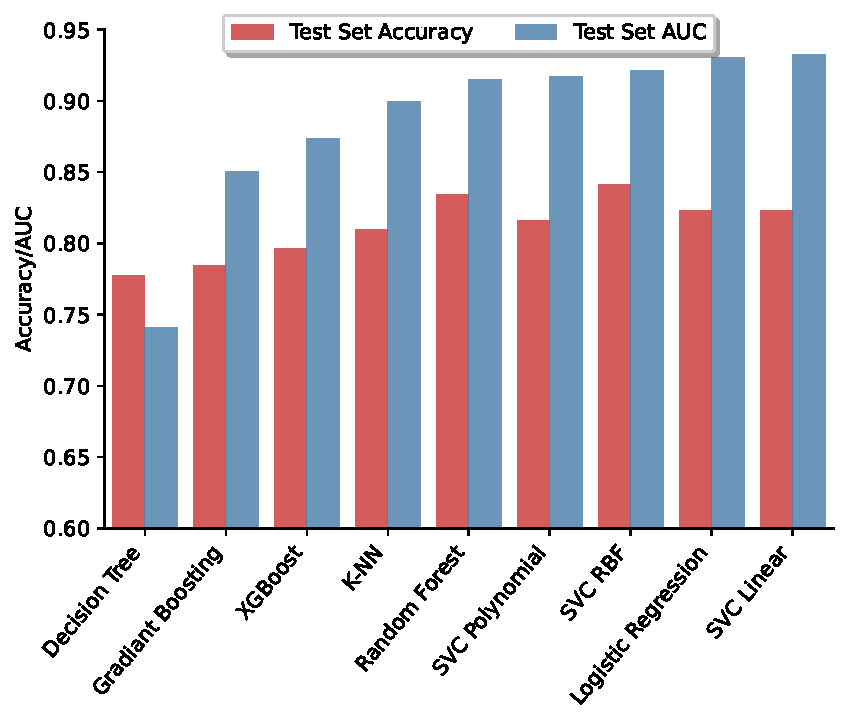
\includegraphics[width=0.65\linewidth]{Models AUC 5 mirs CV}
\caption{Area under the receiver operating characteristic curve and accuracy of different models trained with AUC-selected miRNAs.}\label{fig:AUCmodels}
\end{figure}


\begin{table}
\centering
\caption{AUC-ROC and accuracy for SVM with the linear and RBF kernels as the best models trained with miRNAs selected based on their AUC-ROC on the train and test sets before and after hypertuning}
\label{tab:AUCML}
\begin{tabular}{cccccc}
\toprule
\multicolumn{2}{c}{} & \multicolumn{2}{c}{Preset parameters} & \multicolumn{2}{c}{Hypertuned} \\
\cmidrule(lr){3-4} \cmidrule(lr){5-6}
Model & Metrics & Train & Test & Train & Test\\
\midrule
SVM-linear & AUC-ROC & 0.91 & 0.93 & 0.93 & 0.92\\
& Accuracy & 0.85 & 0.82 & 0.90 & 0.88\\
SVM-RBF & AUC-ROC & 0.90 & 0.92 & 0.96 & 0.96\\
& Accuracy & 0.86 & 0.84 & 0.96 & 0.94\\
\bottomrule
\end{tabular}
\end{table}


\section{Discussion}\label{discussion}

The prevalence of MI can lead to high mortality rates in the clinical
setting. However, early diagnosis and the application of suitable
treatment protocols can reduce mortality and improve MI prognosis
(\cite{CVD, 17, 18}). Studies have suggested that changes in miRNA expression
may play a significant role in the progression of MI and the subsequent
remodeling \cite{23}. It is believed that miRNA
expression is altered during the various biological processes correlated
with MI within the myocardium or other related tissues \cite{24}. Although several studies have focused on examining free
circulating miRNAs in serum samples for the detection of cardiac tissue
injuries \cite{11-15}, more information is needed to fully
comprehend the miRNAs found in different blood subcomponents, such as
plasma, platelets, and PBMCs. Based on previous findings, PBMCs play a
crucial role in the destabilization and rupture of plaques as well as in
the initial inflammatory reactions in individuals experiencing
myocardial infarction (MI) \cite{Meder6, Meder23}.
Moreover, PBMCs have specific miRNA profiles that are altered under
certain pathological conditions, making them great candidates as disease
biomarkers \cite{Meder6}.

PBMCs can respond to several insulting conditions, such as MI, in the
shortest possible time with notable changes in their miRNA profile
\cite{Meder6}. Considering their regulatory roles, subtle
changes in the transcription of miRNAs can be monitored even before
alterations in mRNA and protein levels \cite{miR}. These
features make miRNAs a valid early-stage diagnostic tool for the
detection of minor and major cell injuries. To date, few studies have
compared the miRNA profiles in PBMCs from patients with MI and other
CADs and healthy samples to find a robust set of identical miRNAs to
differentiate these pathological conditions.

In this study, we combined three GEO datasets for healthy, CAD, and MI
samples. Having these sample sets alongside bioinformatics analysis and
ML methods enabled us to identify potential biomarker sets and effective
therapeutic targets. The results of the DEG analysis (Table
~\ref{tab:DEGstab} and Figure~\ref{fig:venn}) prove the close
relationship between the MI and CAD samples. Interestingly, functional
enrichment analysis demonstrated that DEGs in both CAD/healthy and
MI/healthy were strongly correlated with the immune cell response, which
is a major part of PBMCs. Two sets of miRNAs were selected as biomarker
sets for sample classification. miR-21; miR-32; and miR-186 were
selected as differentially expressed miRNAs, and miR-186; miR-21;
miR-29a; miR-197; and miR-296 were selected based on their AUC-ROC
values. As shown in Figure~\ref{fig:miRROC}, all miRNAs selected with
both approaches had AUC-ROCs $> 0.9$ for isolating healthy and
not-healthy samples except for miR-296 and miR-29a. The data confirmed
that the real challenge was to classify CAD and MI samples because of
the close overlap. Of the six miRNAs under investigation in both
approaches, except for miR-32, all miRNAs had an AUC-ROC $> 0.8$ for
the discrimination of CAD and MI samples. As expected, the high AUC-ROC
values of the miRNAs confirmed their high potential as biomarkers.

ML models trained with miRNA sets selected by both DEG and AUC-ROC
approaches, showed better classification performance than each miRNA. To
avoid unwanted complexity and poor predictive values, a two-layer
architecture was designed. The first layer was used to discriminate
between healthy and not-healthy samples, and the second layer was was
used to separate CAD from MI candidates. As expected, in both
approaches, a hypertuned SVM model could flawlessly separate healthy and
not-healthy samples using distinct miRNA sets. ML models are also
capable of effectively separating CAD from MI patients. Although both
miRNA sets had nearly the same AUC-ROC using the best model, their
accuracy, sensitivity, and specificity were different. The model trained
with AUC-selected miRNAs showed better performance in all predictive
values, which is logical because of the higher number of miRNAs in the
set.

Numerous studies have reported that different biological processes can
affect the miRNA expression in PBMCs. However, the exact role of miRNAs
in the function of immune cells and the correlation between specific
pathological conditions and miRNA profiles remain controversial. Several
studies have proven the activation of particular miRNA types in PBMCs
under cardiovascular events \cite{296}. For instance, there is
evidence that elevation of miR-186 suppresses the expression of
cystathionine-$\gamma$-lyase, leading to the subsequent secretion of
pro-inflammatory cytokines and cellular lipid accumulation. In addition,
macrophage-derived miR-186 may promote atherosclerotic plaque formation
\cite{186}. In line with this claim, we found that miR-186 was
up-regulated in both CAD and MI candidates compared to their control
counterparts. Surprisingly, the obtained data indicated that the
expression of miR-186 was higher in patients with CAD than in patients
with MI (Figure~\ref{fig:Expall}). Specifically, miR-186 was the only
differentially expressed miRNA between CAD and MI, with a clear
up-regulation in CAD, indicating its main role in the promotion of
atherosclerosis.

As mentioned before, miR-21 was also up-regulated in both MI and CAD
patients compared to healthy controls. Moreover, the expression value of
miR-21 was significantly higher in the MI group than in the CAD group
(Table~\ref{tab:mirExptable}). It is thought that the up-regulation of
miR-21 in PBMCs is a compensatory reaction to reduce the T$_{reg}$
lymphocyte number in response to the reduction in TGF$\beta1$
secretion into the plasma through a TGF$\beta1$/smad-independent
pathway. In line with the previous and present data, miR-21 can modulate
the activity of PBMCs following the occurrence of cardiovascular
diseases \cite{21}.

Recent data have supported the elevation of miR-32 levels in CAD samples
with calcification of the coronary artery. Notably, miR-32 promotes
vascular smooth muscle calcification in mice by controlling the activity
of several proteins, including bone morphogenetic protein-1,
runt-related transcription factor-2 (RUNX2), osteopontin, and
bone-specific phosphoprotein matrix GLA protein \cite{32-2}.
Likewise, some reports are associated with the activity of miR-32 in
PBMCs in several pathologies \cite{magic, 32}. The
exact role of miR-32 in PBMCs after cardiovascular events remains
unclear.

Molecular analyses have indicated the regulatory role of miRNAs selected
using the AUC-ROC approach in PBMCs after a cardiovascular event. The
biological importance of two common miRNAs in the DEGs and AUC-ROC
approaches, miR-21 and miR-186, have already been discussed. Based on
numerous reports, miR-29a can be activated in different diseases \cite{29aa}. Data analysis indicated that
miR-29a was significantly up-regulated in CAD patients compared to the
healthy and MI groups (Table~\ref{tab:mirExptable}). Increased miR-29a
is associated with the progression of atherosclerosis, and the
combination of miR-29a and ox-LDL has been suggested as a valid
biomarker set for paraclinical classification \cite{29a}.
However, the role of miR-29a in the function of PBMCs from patients with
CAD has not been thoroughly examined.

The data indicated that miR-197 was significantly up-regulated in both
the CAD/healthy and MI/healthy groups. Previous studies have
demonstrated that miR-197 may play a crucial role in controlling the
anti-inflammatory response of IL-35 by influencing the secretion of
cytokines that can either promote or suppress inflammation, the ratio of
M1/M2 macrophages, and the proliferation of T$_{reg}$ lymphocytes,
which are responsible for suppressing immune responses \cite{197}. Alongside our findings, it can be concluded that miR-197 could be
a useful diagnostic tool for predicting adverse cardiovascular events.

The findings of this study demonstrate the potential of miR-296 as a
biomarker with high discriminatory power to distinguish between samples
from individuals with MI and CAD. MiR-296 has been identified as a key
regulator in the development and advancement of atherosclerosis by
controlling the expression of target genes associated with various
biological processes, including angiogenesis, cholesterol metabolism,
inflammation, cellular proliferation, hypertension, and apoptosis \cite{296}. In a previous study, miR-296 expression levels were found
to be significantly increased in the PBMCs of CAD patients compared to
healthy controls, suggesting its involvement in regulating
proinflammatory cytokines such as IL-6 and TNF-$\alpha$ \cite{296a}. These findings suggested that miR-296 may have a significant
impact on the pathogenesis of atherosclerosis and could potentially
serve as a diagnostic biomarker for CAD or MI.
 

\section{Conclusion}\label{conclusion}

In summary, we derived a set of miRNA biomarkers by comparing MI samples
with both healthy and CAD samples. We found that the SVM model performed
best in both the first layer, which separated healthy and unhealthy
samples, and the second layer, which classified the MI/CAD samples. The
set of miRNAs selected based on their AUC-ROC values performed better in
the second layer. Overall, our two-layer structure achieved an accuracy
of 0.96. This demonstrates the potential of combining bioinformatics and
machine learning techniques to identify novel biomarkers and gain a
deeper understanding of myocardial infarction.

\section{Abbreviations}\label{abbreviations}

\begin{description}
  \item \textbf{CVD}: Cardiovascular disease
  \item \textbf{MI}: Myocardial infarction
  \item \textbf{cTn}: Cardiac troponin
  \item \textbf{miRNA}: microRNA 
  \item \textbf{PBMC}: Peripheral blood mononuclear cell 
  \item \textbf{ML}: Machine learning 
  \item \textbf{GEO}: Gene Expression Omnibus 
  \item \textbf{PCA}: Principal component analysis 
  \item \textbf{RLE}: Relative log expression 
  \item \textbf{FDR}: False discovery rate 
  \item \textbf{DEG}: Differentially expressed gene
  \item \textbf{KEGG}: Kyoto Encyclopedia of Genes and Genomes 
  \item \textbf{GO}: Gene Ontology  
  \item \textbf{BP}: Biological process 
  \item \textbf{CC}: Cellular component 
  \item \textbf{MF}: Molecular function 
  \item \textbf{SVM}: Support vector machine 
  \item \textbf{LR}: Logistic regression 
  \item \textbf{RF}: Random forests
  \item \textbf{kNN}: K-nearest neighbor 
  \item \textbf{GB}: Gradient boosting 
  \item \textbf{XGB}: XGBoost 
  \item \textbf{DT}: Decision tree 
  \item \textbf{AUC-ROC}: Area under the receiver operating characteristic curve 
\end{description}

\backmatter

%%===================================================%%
%% For presentation purpose, we have included        %%
%% \bigskip command. please ignore this.             %%
%%===================================================%%
\bigskip
\begin{flushleft}%
Editorial Policies for:

\bigskip\noindent
Springer journals and proceedings: \url{https://www.springer.com/gp/editorial-policies}

\bigskip\noindent
Nature Portfolio journals: \url{https://www.nature.com/nature-research/editorial-policies}

\bigskip\noindent
\textit{Scientific Reports}: \url{https://www.nature.com/srep/journal-policies/editorial-policies}

\bigskip\noindent
BMC journals: \url{https://www.biomedcentral.com/getpublished/editorial-policies}
\end{flushleft}


\bibliography{sn-article.bib}% common bib file
%% if required, the content of .bbl file can be included here once bbl is generated




\section*{Declarations}


\subsection*{Funding}
This is a report of result from Ph.D. thesis registered in Tabriz University of Medical Sciences with the Number 66372 . This work was extracted from Mehrdad Samadishadlou's thesis titled “Developing and manufacturing of a paper-based Nanobiosensor in order to diagnosing myocardial infarction using a set of blood microRNAs”.

\subsection*{Competing interests}
The authors declare that they have no competing interests.

\subsection*{Ethics approval}
The study was approved by the research ethics committee of Tabriz University of Medical Sciences (approval ID: IR.TBZMED.VCR.REC.1399.388, date of approval: 2021/1/11).

\subsection*{Consent for publication}
All authors gave consent for the publication of the article.

\subsection*{Availability of data and materials}
The datasets generated and/or analysed during the current study are available in the Gene Expression Omnibus (GEO, \url{https://www.ncbi.nlm.nih.gov/geo/}), reference numbers GSE59867, GSE56609 and GSE54475. All data generated or analysed during this study are included in this published article.

\subsection*{Authors' contributions}

F.B. and K.K. conceived the idea and coordinated the project.
M.S. researched, collected the data, performed the analyzes, assembled the results, and drafted the manuscript.
Z.P. and M.E.contributed to data analyze.
Ç.B.A. was foreign supervisor and collaborator.
F.B., R.R. and K.K. edited and revised the manuscript.
F.B. and K.K. are author responsible for contact and ensures communication.

\end{document}
